\documentclass{eth-semester-report}

\usepackage{subcaption}
\usepackage[colorinlistoftodos,textsize=small]{todonotes}

% Disable automatic hyphenation across the whole document.
\hyphenpenalty=10000
\exhyphenpenalty=10000

% --- Metadata (edit before submission) ---
\reportTitle{Cloud-Aware Learning-Based Attitude Control for Rainforest Earth Observation}
\reportAuthor{C\'edric Grieder}
\reportSupervisor{Prof.\ Dr.\ Marco Hutter (ETH RSL); Alejandro Torrents Rufas \& Mathias Burkhalter (Beyond Gravity)}
\reportInstitute{Robotic Systems Lab, ETH Z\"urich \textbar\ Semester project at Beyond Gravity}
\reportProgram{MSc Mechanical Engineering, ETH Z\"urich}

\begin{document}

\maketitle
\thispagestyle{empty}
\null
\newpage

\section*{Abstract}
\addcontentsline{toc}{section}{Abstract}
Satellite imaging of tropical rainforests is limited by persistent cloud cover.
Conventional controllers image every target on a fixed pointing schedule, regardless of cloud conditions.
Shutter budget and downlink capacity are wasted on cloud-obscured frames scientists cannot use.
An autonomous pointing and scheduling policy that reacts to onboard camera observations would use those resources more efficiently.

Because that idea appears straightforward, this work asks a narrower question:
what reward shaping and action-space design are required to train such a policy in simulation?
We build a reproducible platform for that investigation: single-axis attitude dynamics, ray-tracing cameras, parameterised cloud primitives, and a multi-phase safety controller.
A deterministic sequential-target overflight policy serves as the comparison baseline.
Two off-policy reinforcement-learning algorithms are trained and evaluated: Soft Actor-Critic and Maximum a Posteriori Policy Optimisation.

The experiments show that the problem is not trivial in practice.
Reward structure, how the agent commands attitude, and correct algorithm implementation each had to be resolved before useful behaviour emerged.
Both algorithms eventually develop selective shuttering absent in the deterministic baseline, but reliable mission-level gains over that baseline were not established within the semester scope.

The study is limited to a 2D single-pass orbital model.
Attitude safety constraints are enforced throughout.
Flight hardware, multi-orbit planning, and three-dimensional operations are out of scope.


\newpage
\tableofcontents
\newpage

\section*{Nomenclature}
\addcontentsline{toc}{section}{Nomenclature}
% Physical constants and notation used in simulation and learning experiments.
% Numeric values match the implementation at report revision; source locations are in the Appendix.

\subsection{Abbreviations}
\begin{tabular}{p{0.12\linewidth}p{0.80\linewidth}}
  \toprule
  Abbreviation & Definition \\
  \midrule
  CNN & Convolutional neural network (vision observation encoder) \\
  EO & Earth observation \\
  FOV & Field of view \\
  GSD & Ground sample distance \\
  LLA & Latitude, longitude, altitude (geodetic coordinates) \\
  LOS & Line of sight \\
  MLP & Multilayer perceptron (scalar observation branch) \\
  SAC & Soft Actor-Critic \\
  MPO & Maximum \emph{a posteriori} policy optimization \\
  OBC & On-board computer \\
  PD & Proportional--derivative (pointing controller) \\
  RL & Reinforcement learning \\
  RW & Reaction wheel \\
  WGS84 & World Geodetic System 1984 (reference ellipsoid) \\
  \bottomrule
\end{tabular}

\subsection{Symbols}
\begin{tabular}{p{0.14\linewidth}p{0.78\linewidth}}
  \toprule
  Symbol & Meaning \\
  \midrule
  $R_{\mathrm{E}}$ & Mean Earth radius (orbital geometry) \\
  $\mu$ & Earth gravitational parameter \\
  $h$ & Orbit altitude above mean Earth radius \\
  $I_{\mathrm{sat}}$ & Spacecraft moment of inertia (2D model: $I_{zz}$) \\
  $\boldsymbol{\tau}$ & Reaction-wheel torque command [N\,m] (scalar in the 2D kernel) \\
  $\theta_{\mathrm{orb}}$ & True anomaly of the satellite (= orbit-plane angle in circular orbit) \\
  $\theta_{\mathrm{body}}$ & Body $z$-axis angle in the orbit disk \\
  $\omega_{\mathrm{sat}}$, $\omega_{\mathrm{w}}$ & Spacecraft body rate and wheel speed \\
  $f_{\mathrm{cloud}}$ & Primary-camera cloud-blocked fraction along the sensor strip \\
  \bottomrule
\end{tabular}

\subsection{Physical and simulation constants}
Unless noted, values are fixed inputs; $h$ and cloud layouts are randomized per episode (Table~\ref{tab:constants-mission}).

\begin{table}[htbp]
  \centering
  \renewcommand{\arraystretch}{1.3}
  \caption{Earth, orbit, and spacecraft parameters.}
  \label{tab:constants-earth-spacecraft}
  \small
  \begin{tabular}{llS[table-format=4.4]l}
    \toprule
    {Quantity} & {Symbol} & {Value} & {Unit / note} \\
    \midrule
    Mean Earth radius & $R_{\mathrm{E}}$ & 6371.0088 & \si{\kilo\meter} \\
    Gravitational parameter & $\mu$ & 398600.4418 & \si{\kilo\meter\cubed\per\second\squared} \\
    Geodetic model & --- & \multicolumn{2}{l}{WGS84 ellipsoid (surface / LOS)} \\
    Orbit altitude (episode) & $h$ & \multicolumn{2}{l}{uniform on $[\SI{510}{\kilo\meter},\,\SI{570}{\kilo\meter}]$} \\
    Satellite mass & $m_{\mathrm{sat}}$ & 250 & \si{\kilogram} \\
    Moment of inertia (3D) & $I_{xx}, I_{yy}, I_{zz}$ & \multicolumn{2}{l}{16.6, 21.7, 31.2 \si{\kilogram\meter\squared}} \\
    Moment of inertia (2D sim.) & $I_{\mathrm{sat}}$ & 31.2 & \si{\kilogram\meter\squared} ($I_{zz}$) \\
    RW max torque & $\tau_{\max}$ & 0.1 & \si{\newton\meter} \\
    RW max momentum & $H_{\max}$ & 0.4 & \si{\newton\meter\second} \\
    Star-tracker rate limit & --- & 3 & \si{\degree\per\second} \\
    Off-nadir hard limit & --- & 45 & \si{\degree} \\
    \bottomrule
  \end{tabular}
\end{table}

\begin{table}[htbp]
  \centering
  \renewcommand{\arraystretch}{1.3}
  \caption{Camera and simulation timing.}
  \label{tab:constants-camera-sim}
  \small
  \begin{tabular}{llS[table-format=4.0]l}
    \toprule
    {Quantity} & {Symbol} & {Value} & {Unit / note} \\
    \midrule
    Sensor resolution & --- & \multicolumn{2}{l}{9344 $\times$ 7000 pixels (cross $\times$ along)} \\
    Pixel pitch & --- & 3.2 & \si{\micro\meter} \\
    Focal length & $f$ & 1067 & \si{\milli\meter} \\
    Exposure time & $t_{\mathrm{exp}}$ & 100 & \si{\micro\second} \\
    Simulation step & $\Delta t$ & 1.5 & \si{\second} \\
    Max captures per orbit & --- & 10 & shutter budget (resource proxy) \\
    \midrule
    \multicolumn{4}{l}{\textit{Secondary wide-angle camera}} \\
    Sensor resolution & --- & \multicolumn{2}{l}{5312 $\times$ 2988 pixels} \\
    Pixel pitch & --- & 1.55 & \si{\micro\meter} \\
    Vertical FOV & --- & 70 & \si{\degree} \\
    Boresight tilt from nadir & --- & 25 & \si{\degree} \\
  \bottomrule
  \end{tabular}
\end{table}

\begin{table}[htbp]
  \centering
  \renewcommand{\arraystretch}{1.3}
  \caption{Mission profile and reward scales (default training configuration).}
  \label{tab:constants-mission}
  \small
  \begin{tabular}{p{0.40\linewidth}p{0.52\linewidth}}
    \toprule
    Quantity & Value / range \\
    \midrule
    Target grid & 50 areas, \SI{15}{\kilo\meter} extent, \SI{40}{\kilo\meter} spacing along corridor \\
    Cloud patches per episode & uniform integer in $[15,\,30]$ along corridor \\
    Cloud horizontal extent & \SIrange{1}{80}{\kilo\meter} \\
    Cloud base altitude & \SIrange{4}{12}{\kilo\meter} \\
    Cloud thickness & \SIrange{1}{16}{\kilo\meter}; top capped at \SI{20}{\kilo\meter} \\
    Capture reward weight & $w_{\mathrm{capture}} = 100$ \\
    Optimal / threshold ground range & $d_{\mathrm{op}} = \SI{400}{\kilo\meter}$, $d_{\mathrm{th}} = \SI{1500}{\kilo\meter}$ \\
    Viewing-distance outer gate & \SI{2500}{\kilo\meter} \\
    \bottomrule
  \end{tabular}
\end{table}


\newpage

\section{Introduction}
\subsection{Motivation}
Climate and environmental science depend on repeat optical imaging of regions such as tropical rainforests, where cloud cover is frequent and unpredictable at the timescale of a satellite pass.
Mission operators today often rely on deterministic strategies with fixed nadir attitude and pre-planned shutter times that treat every target along a ground track equally.
When clouds occlude the line of sight, those strategies still consume onboard memory and downlink budget on low-value frames, while scientists lose observations that may not be recoverable on the next pass.
The cost is therefore threefold: reduced science yield, wasted capture capacity, and unnecessary actuator activity from indiscriminate pointing and slewing.

Autonomous onboard decision-making is motivated by latency: ground-in-the-loop replanning cannot react to the cloud layout actually present during the pass.
Both \emph{when} to expose the shutter and \emph{how} to orient the spacecraft for maximal image quality therefore matter, and they must respect attitude safety limits on reaction-wheel use and pointing envelopes.
From the outside, the required behaviour looks straightforward: use onboard camera feedback to skip cloud-occluded targets and capture only when the view is clear.
This report treats that apparent simplicity as the starting point and asks what training design is actually required to reach it.

The specific orbit geometry is not tied to a polar versus equatorial regime.
Any circular orbit viewed at the instant of overflight is equivalent for the control problem posed here.

\paragraph{Current operational process.}
In a typical Earth-observation mission today, domain scientists compile a list of target areas they wish to image and submit it to mission control.
The ground segment then builds an observation schedule: it checks which targets fall within the satellite's ground track on upcoming passes, verifies observable constraints such as solar illumination and off-nadir angle limits, and uplinks a fixed command sequence.
This process works well for constraints that can be predicted from orbital mechanics.
Cloud cover, however, cannot be scheduled out: the weather state at the moment of overflight is unknown at planning time, and the uplinked schedule cannot be modified during the pass.
The satellite therefore executes its pre-planned capture sequence regardless of what the cameras actually see, consuming onboard storage, electrical power, downlink capacity, and attitude-control effort on frames that may be entirely cloud-occluded \citep{ferrari2024ssp}.

\subsection{Intended solution concept}
\label{sec:solution-concept}

Today's operational process is ground-planned: the capture list is fixed before the pass, and uplink latency is too large for cloud-aware replanning during overflight.
Under that paradigm a forward-looking sensor has little operational value, because the satellite cannot act on what it sees ahead.
Consequently, current missions typically do not fly a dedicated lookahead imager for in-pass scheduling.

An onboard scheduling agent changes that premise.
If capture decisions are made during the pass, the agent needs information about upcoming targets and cloud conditions \emph{before} those scenes enter the primary imaging window.
Otherwise it can react only when a target is already under the science boresight, which is too late for useful opportunity selection under a limited shutter budget.

The primary payload is a narrow-field science camera (hyperspectral-class in the mission concept).
Pointing that instrument forward would still cover only a thin along-track strip, so it is a poor lookahead sensor for surveying multiple upcoming opportunities.
This study therefore adds a second, forward-tilted wide-angle (fisheye) camera that observes the corridor ahead while the primary camera remains dedicated to science capture near nadir
(Table~\ref{tab:constants-camera-sim}; $\SI{70}{\degree}$ along-track FOV, $\SI{25}{\degree}$ prograde tilt).
Figure~\ref{fig:concept-lookahead} illustrates this sensing geometry on a representative along-track pass.

\begin{figure}[htbp]
  \centering
  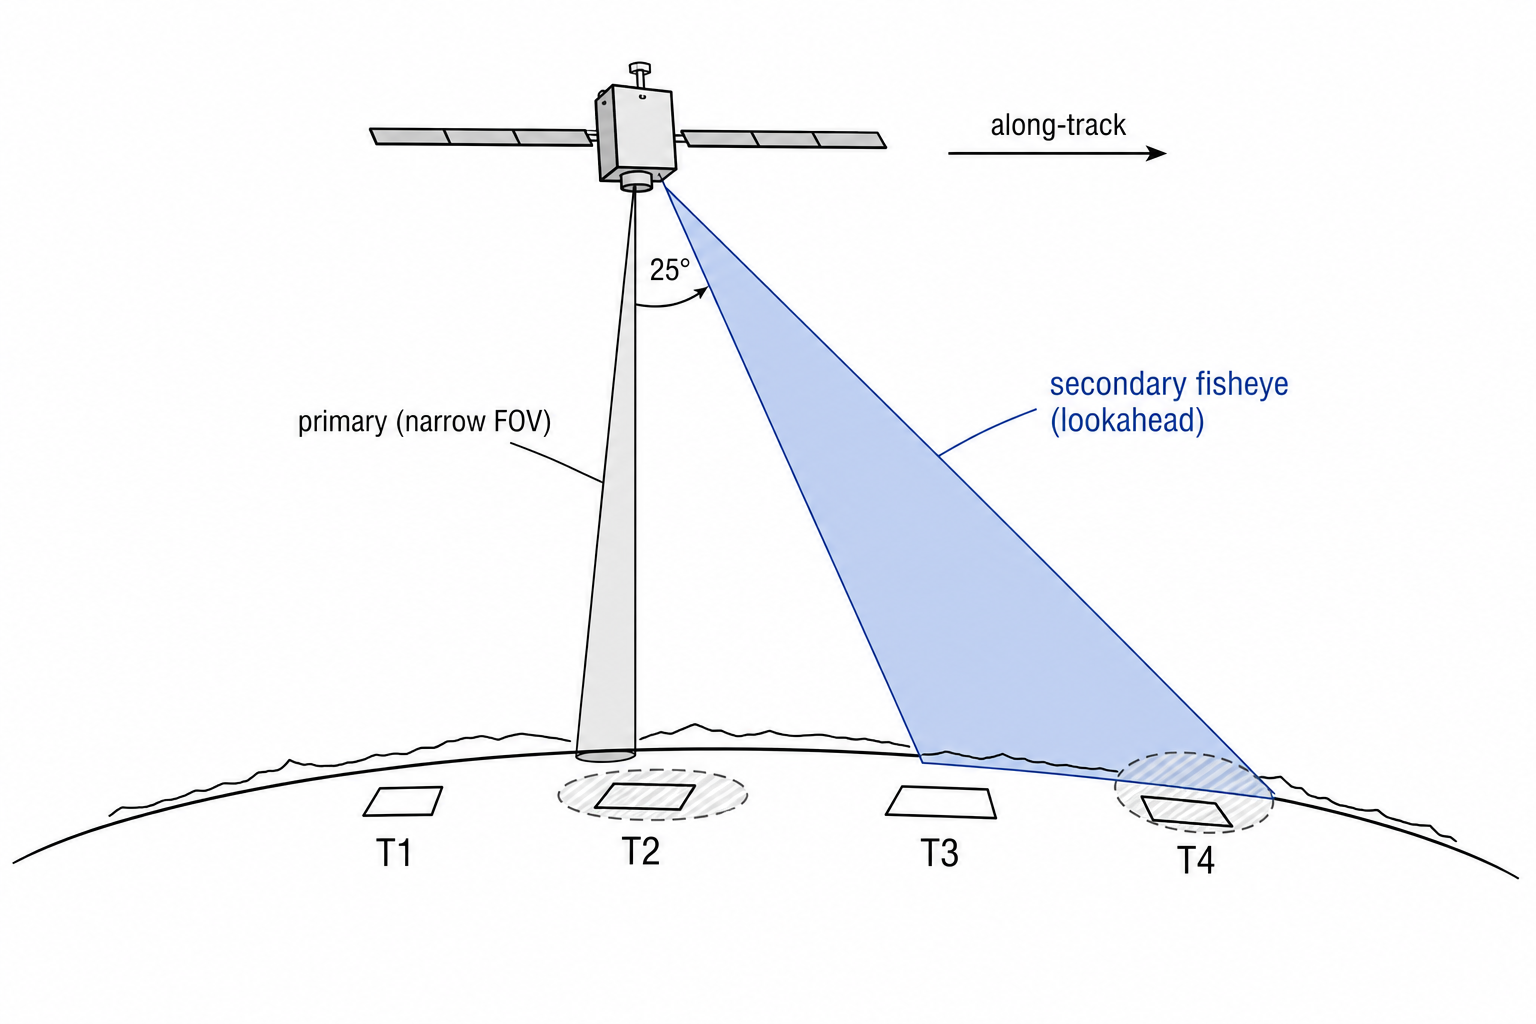
\includegraphics[width=0.92\linewidth]{figures/fig_concept_lookahead_eth.png}
  \caption{Lookahead sensing geometry.
    The narrow primary camera images near nadir while a forward-tilted fisheye observes upcoming targets along-track before they enter the primary footprint
    ($\SI{25}{\degree}$ prograde tilt; Table~\ref{tab:constants-camera-sim}).}
  \label{fig:concept-lookahead}
\end{figure}

Lookahead sensing is not unique to a fisheye.
Alternatives include cloud or weather products from other satellites, relayed via the ground segment or cross-link, and those products need not be image-shaped at all.
We evaluate the onboard fisheye approach because it is deployment-feasible on a single spacecraft and avoids network effects and external data dependencies:
as long as the satellite has power and a downlink path for the science data it produces, the scheduling loop can operate from its own sensors.

The intended decision process is sequential opportunity selection under scarcity.
The fisheye reveals clear and cloud-occluded candidates ahead of the primary footprint; an onboard policy ranks those imaging opportunities and spends the limited shutter budget (proxying storage, downlink capacity, and actuator effort) on high-value clear captures rather than executing a fixed pre-planned schedule.
This report then asks a narrower training question: which reward shaping and action-space designs make that selective behaviour learnable in simulation.

\subsection{Research question}
\label{sec:research-question}

Cloud-aware autonomous scheduling is an obvious improvement over fixed pre-planned capture.
The motivating question of this report is therefore not whether such a policy should exist, but how to train one in simulation:
\begin{quote}
  \textbf{What reward shaping and action-space design are sufficient for a reinforcement-learning agent to learn selective pointing and shuttering during a cloud-occluded Earth-observation pass?}
\end{quote}
Capture decisions are sequential and uncertain.
Cloud occlusion, attitude dynamics, and discrete shutter events interact over a single pass, so the design of the learning interface matters as much as the algorithm choice.
The experiments below treat this as a design-space question: which training choices make selective shuttering learnable, and which do not.

\subsection{Related work}
\label{sec:related-work}

Earth-observation satellite scheduling is a well-studied operations-research domain.
Surveys of satellite scheduling problems document how limited onboard storage, downlink, and energy constrain capture opportunities, and how waste of those resources reduces science yield \citep{ferrari2024ssp}.
Much of that literature addresses ground-segment planning over multi-orbit horizons.
The present work instead asks how a single-pass, onboard policy should decide pointing and shuttering when cloud cover is revealed only during the overflight.

Continuous-control reinforcement learning provides candidate algorithms for that onboard layer.
Soft Actor-Critic (SAC) combines off-policy sample reuse with a maximum-entropy objective, which tends to stabilise stochastic continuous control relative to brittle deterministic off-policy methods \citep{haarnoja2018sac}.
Maximum a Posteriori Policy Optimisation (MPO) frames improvement as relative-entropy-constrained policy iteration with separate trust regions on the policy mean and covariance \citep{abdolmaleki2018mpo}.
Both algorithms are used in the experiments below as interchangeable learners over a shared environment and observation stack.

Beyond the policy update, observation structure matters when sensors are heterogeneous.
Integrating state representation learning into deep RL shows that reward alone may not shape a usable embedding when modalities must be fused, and that structured encoders improve sample efficiency and generalisation \citep{bruin2018irl}.
For tabular and numeric inputs specifically, embedding numerical features before mixing outperforms feeding raw scalars through a shallow multilayer perceptron \citep{gorishniy2022revisiting}; that motivation underlies encoder variants that compress structured bearing and mask fields before fusion with vision features.

Prior work therefore covers Earth-observation resource scheduling, stable continuous-control RL, and structured observation encoders.
It does not, however, map which reward shaping and action-space designs are sufficient for cloud-aware shuttering under hard attitude-safety constraints in this simplified Earth-observation setting.
That mapping is the focus of the present report.

\subsection{Deterministic baseline}
\label{sec:baseline-intro}

\begin{figure}[htbp]
  \centering
  \begin{subfigure}[t]{0.32\linewidth}
    \centering
    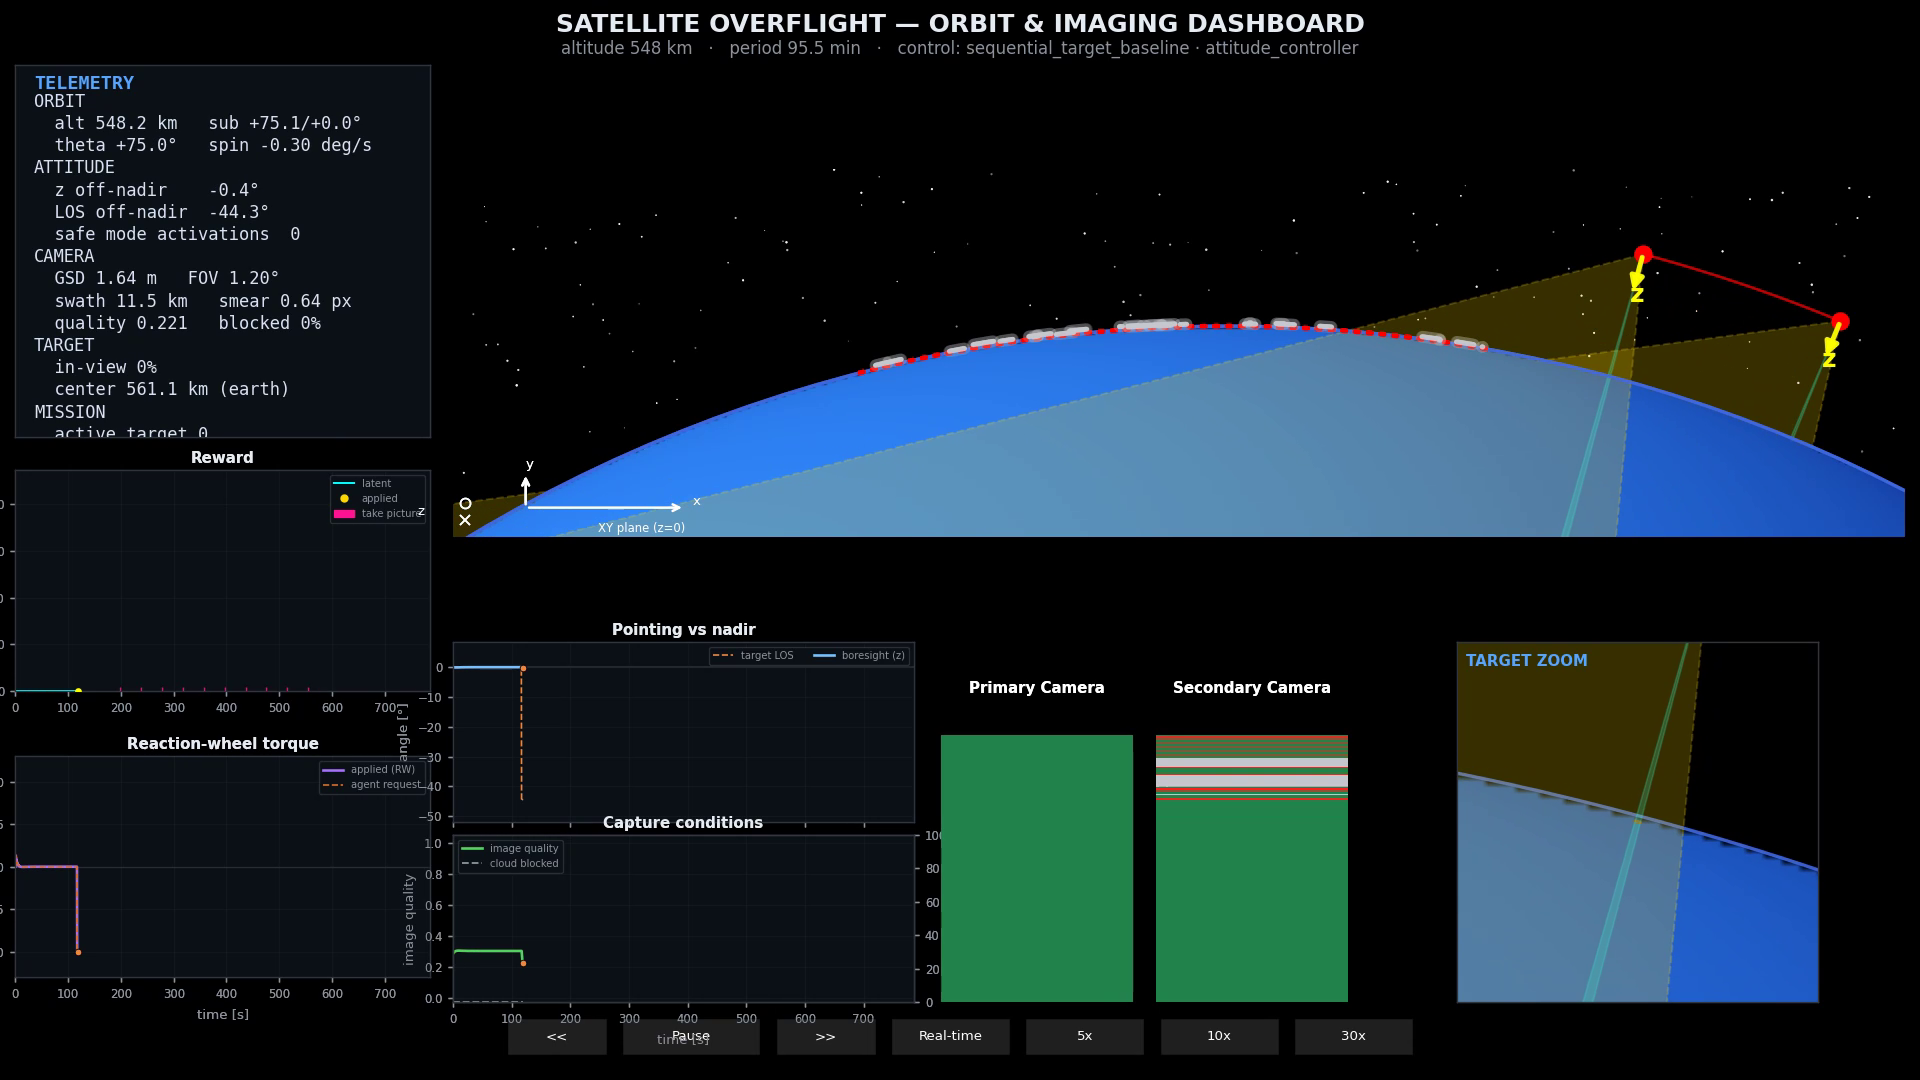
\includegraphics[width=\linewidth]{figures/fig_baseline_phase_approach.png}
    \caption{Approach}
  \end{subfigure}\hfill
  \begin{subfigure}[t]{0.32\linewidth}
    \centering
    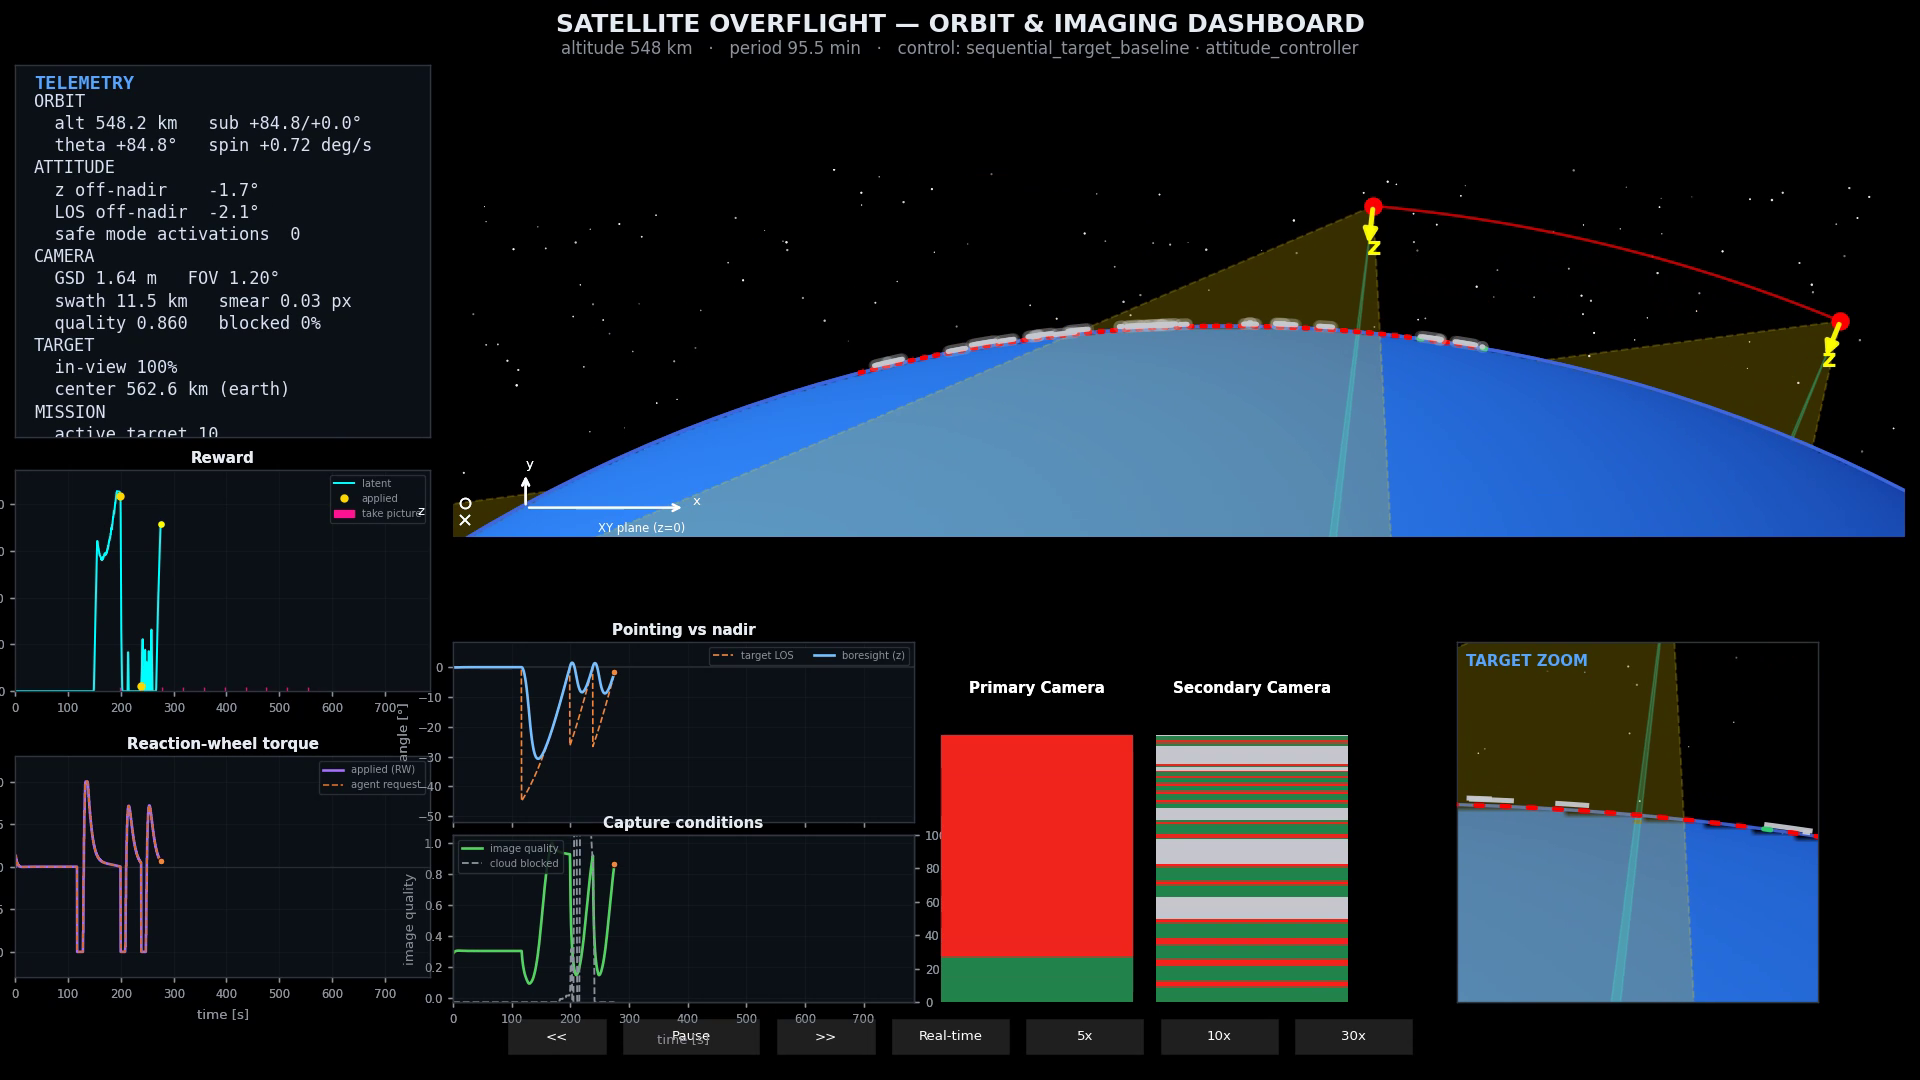
\includegraphics[width=\linewidth]{figures/fig_baseline_phase_point.png}
    \caption{Point}
  \end{subfigure}\hfill
  \begin{subfigure}[t]{0.32\linewidth}
    \centering
    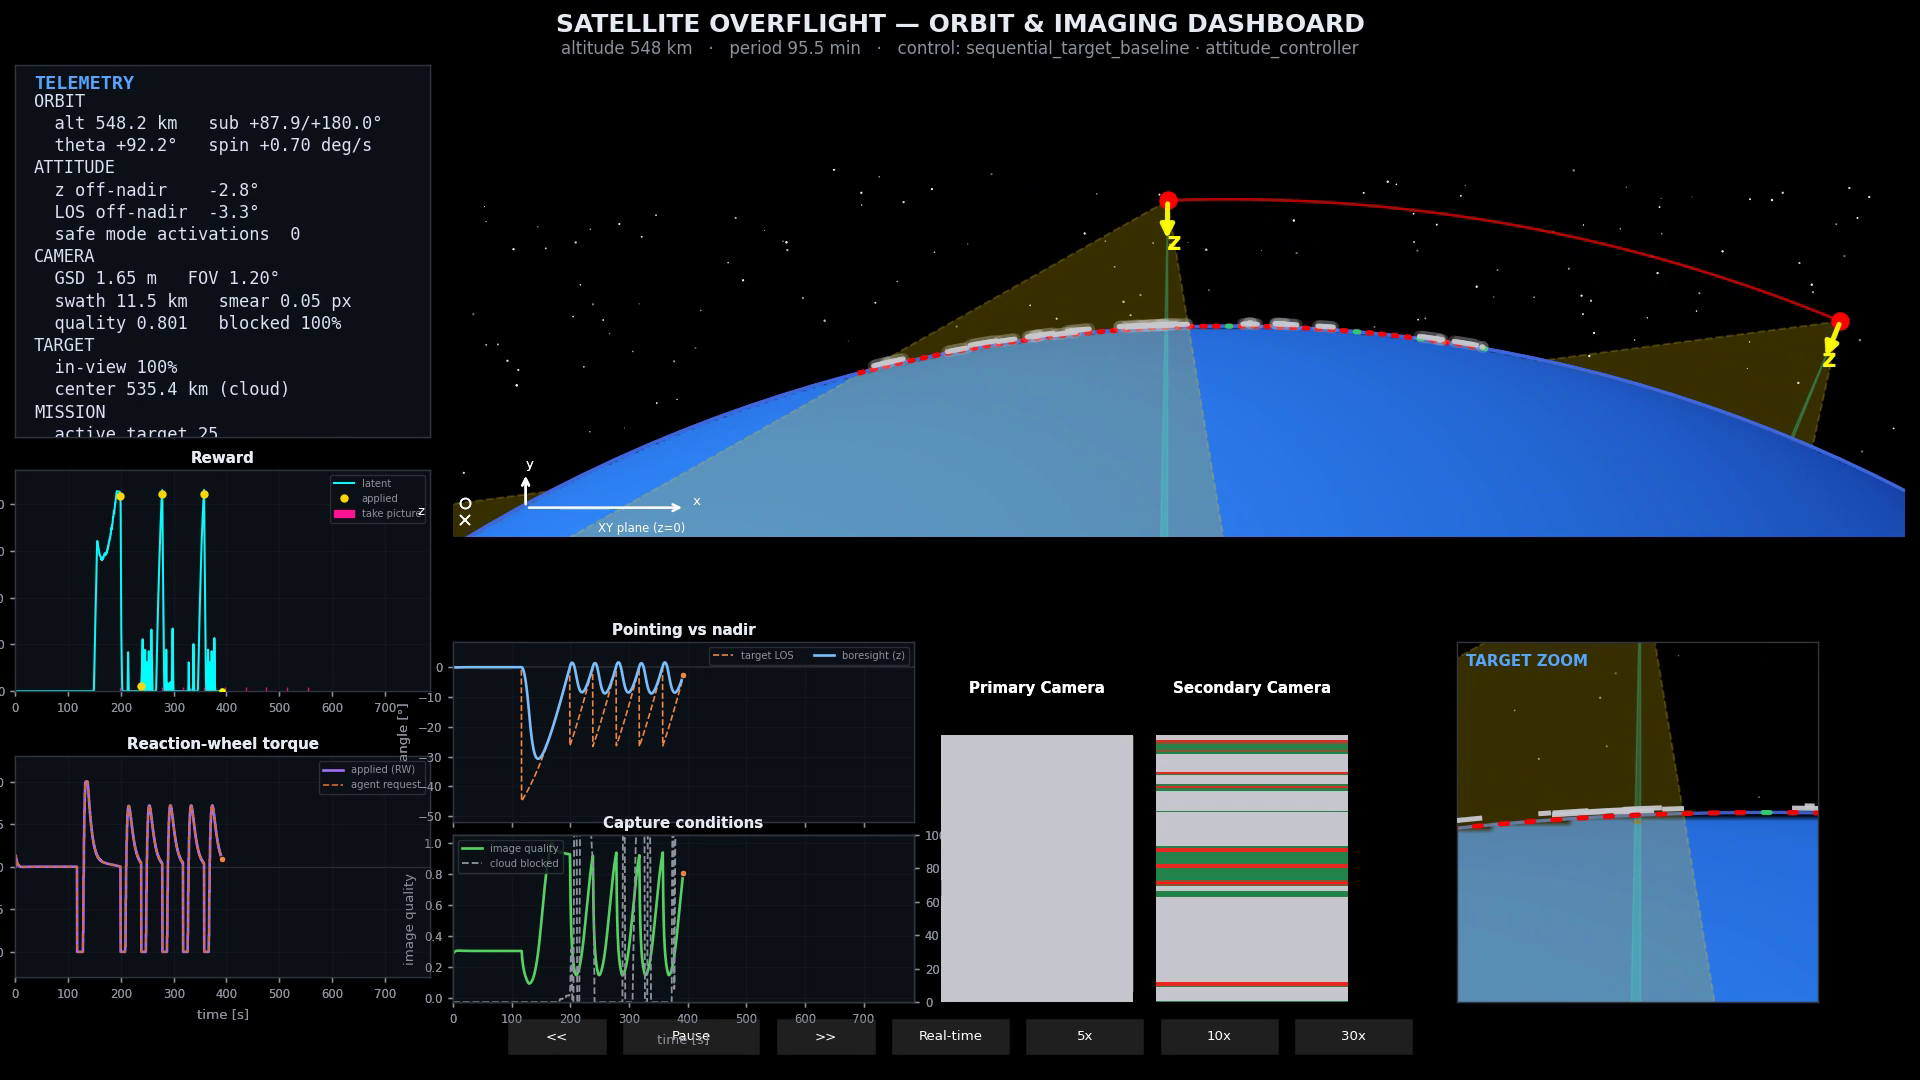
\includegraphics[width=\linewidth]{figures/fig_baseline_phase_capture.png}
    \caption{Capture}
  \end{subfigure}
  \caption{Deterministic baseline overflight (orbit-disk dashboard).
    Left to right: (a)~Approach: nadir coast into the target corridor before the first lock;
    (b)~Point: large off-nadir slew toward the scheduled target bearing;
    (c)~Capture: return to nadir after the first shutter, with high image quality and the reward spike still visible.
    The schedule fires regardless of cloud cover (Table~\ref{tab:baseline-config}).}
  \label{fig:baseline-overflight-phases}
\end{figure}

The reference strategy is a pre-scheduled sequential controller used as the comparison anchor throughout the experiments (Section~\ref{sec:baseline}): an OBC proportional--derivative loop commands target body angles (nadir coast or target bearing) under the same attitude-safety stack as the learned policy, with no cloud awareness and no adaptive capture list (see Table~\ref{tab:baseline-config}).

A real mission is additionally constrained by onboard memory, downlink bandwidth, and energy \citep{ferrari2024ssp}.
We model this resource limit with a \emph{shutter budget}: a hard cap of ten capture actions per episode.
Because the deterministic baseline treats every scheduled target equally, that budget is consumed indiscriminately across clear and cloud-occluded targets alike.
This yields a fixed, predictable observation cadence but wastes capture capacity on frames that are scientifically unusable when a cloud is in the field of view.

\subsection{Scope and simplifications}
\label{sec:scope}

The model deliberately stays close to the control problem while omitting much operational detail: 2D attitude dynamics, basic circular-orbit geometry, physical ray tracing for cameras and clouds, safety arbitration, and single-pass episodes.
It does not model multi-orbit scheduling, flight hardware, or real imagery ingestion.
Illumination conditions are not modelled: all episodes are treated as daytime passes with perfect solar lighting.
This is a deliberate simplification.
Optical Earth observation is not performed at night, and solar geometry only excludes certain orbit geometries rather than driving frame-to-frame image quality during a pass.
Cloud occlusion is a far stronger and more variable image quality constraint within a single pass, and is the focus of this work.
Section~\ref{sec:methods} describes how the question was investigated and lists modelled subsystems explicitly; Discussion states extensions (three-dimensional attitude, richer terrain, stronger RL benchmarks) as logical next steps rather than deliverables of this semester project.

\textbf{Long-term context.}
The intended onboard stack is hierarchical: a mission planner sets observation intent, a learned policy decides when and what to image, and an OBC executes maneuvers through PD pointing under hard attitude-safety limits.
This report maps the learning interface for that scheduling layer, not the full flight stack.
Section~\ref{sec:discussion-architecture} details the control hierarchy and the torque-to-vector action-interface path explored in the experiments.

\subsection{Contributions}
This report documents:
\begin{itemize}
  \item \textbf{Platform.} A simulation-and-learning pipeline with seeded mission randomisation and matched baseline comparison, so that reward and action-space variants are tested under identical cloud and target draws.
  \item \textbf{Design-space study.} A sequence of fourteen experiments that maps which reward terms, action representations, and algorithm choices enable cloud-aware shuttering behaviour, and which do not.
  \item \textbf{Evaluation protocol.} Training and evaluation conventions with a fixed environment seed, baseline-policy buffer seeding, and a deterministic baseline as the comparison anchor.
  \item \textbf{Evidence.} Qualitative and quantitative artefacts from frozen runs, including selective shuttering behaviour in late-training episodes where learning succeeded.
\end{itemize}

The engineering platform and the experimental map are the primary deliverables; mission-level outperformance of the baseline was not established within the semester scope (Section~\ref{sec:discussion}).

\subsection{Report structure}
Section~\ref{sec:solution-concept} states the intended onboard sensing and scheduling concept.
Section~\ref{sec:related-work} situates the work against Earth-observation scheduling surveys and continuous-control reinforcement learning.
Section~\ref{sec:methods} describes the research approach, simulation environment, and learning method.
Section~\ref{sec:experiments} documents the design-space search: which reward and action-space choices were tested and what each revealed.
Section~\ref{sec:results} aggregates the behavioural and return outcomes.
Sections~\ref{sec:discussion} and~\ref{sec:conclusion} interpret the mapped design space, rejected shortcuts, and outlook.
Technical constants are listed in the Nomenclature section; source-code entry points are in the Appendix.


\section{Methods}
\label{sec:methods}

This section describes how the research question (Section~\ref{sec:research-question}) was investigated.
We built a simulation platform and ran a sequence of controlled experiments that varied reward terms, action representation (direct torque versus nadir-relative pointing offset), and learning algorithm.
Each configuration was evaluated against the deterministic baseline (Section~\ref{sec:baseline-intro}) under matched environment draws: same altitude, cloud layout, and target positions per episode.
Success is measured by whether the agent learns a stable policy that uses vision feedback to shutter selectively rather than on every step.

The subsections below document every modelling choice, constant, and algorithm in sufficient detail to reproduce the experiment results.
Numeric values appear in the Nomenclature and in the tables below; repository source locations are listed in the Appendix.

% ─────────────────────────────────────────────────────────────────────────────
\subsection{Environment overview}
\label{sec:env-overview}

The mission is a single-satellite nadir-looking Earth-observation overflight.
One episode represents a single contiguous pass over a ground corridor.

\paragraph{Altitude and orbit.}
The simulation uses a 2D orbit-plane model: the satellite moves as a point on a circle whose true anomaly $\theta_\text{orbit}$ advances at the instantaneous circular orbit rate (in a circular orbit, true anomaly equals orbital angle).
Orbital altitude is sampled uniformly from $[\SI{510}{km},\,\SI{570}{km}]$ per episode; all other geometry scales with altitude, so the choice of specific ground track is arbitrary.

\paragraph{Target corridor.}
Fifty observation targets are placed at fixed positions along a ground corridor directly below the orbit plane.
Their angular positions in the orbit plane are computed once at episode initialisation from the sampled altitude.
The specific geographic location of the corridor is irrelevant: the agent only ever sees orbit-plane angles, cloud fractions, and attitude state.

\begin{figure}[htbp]
  \centering
  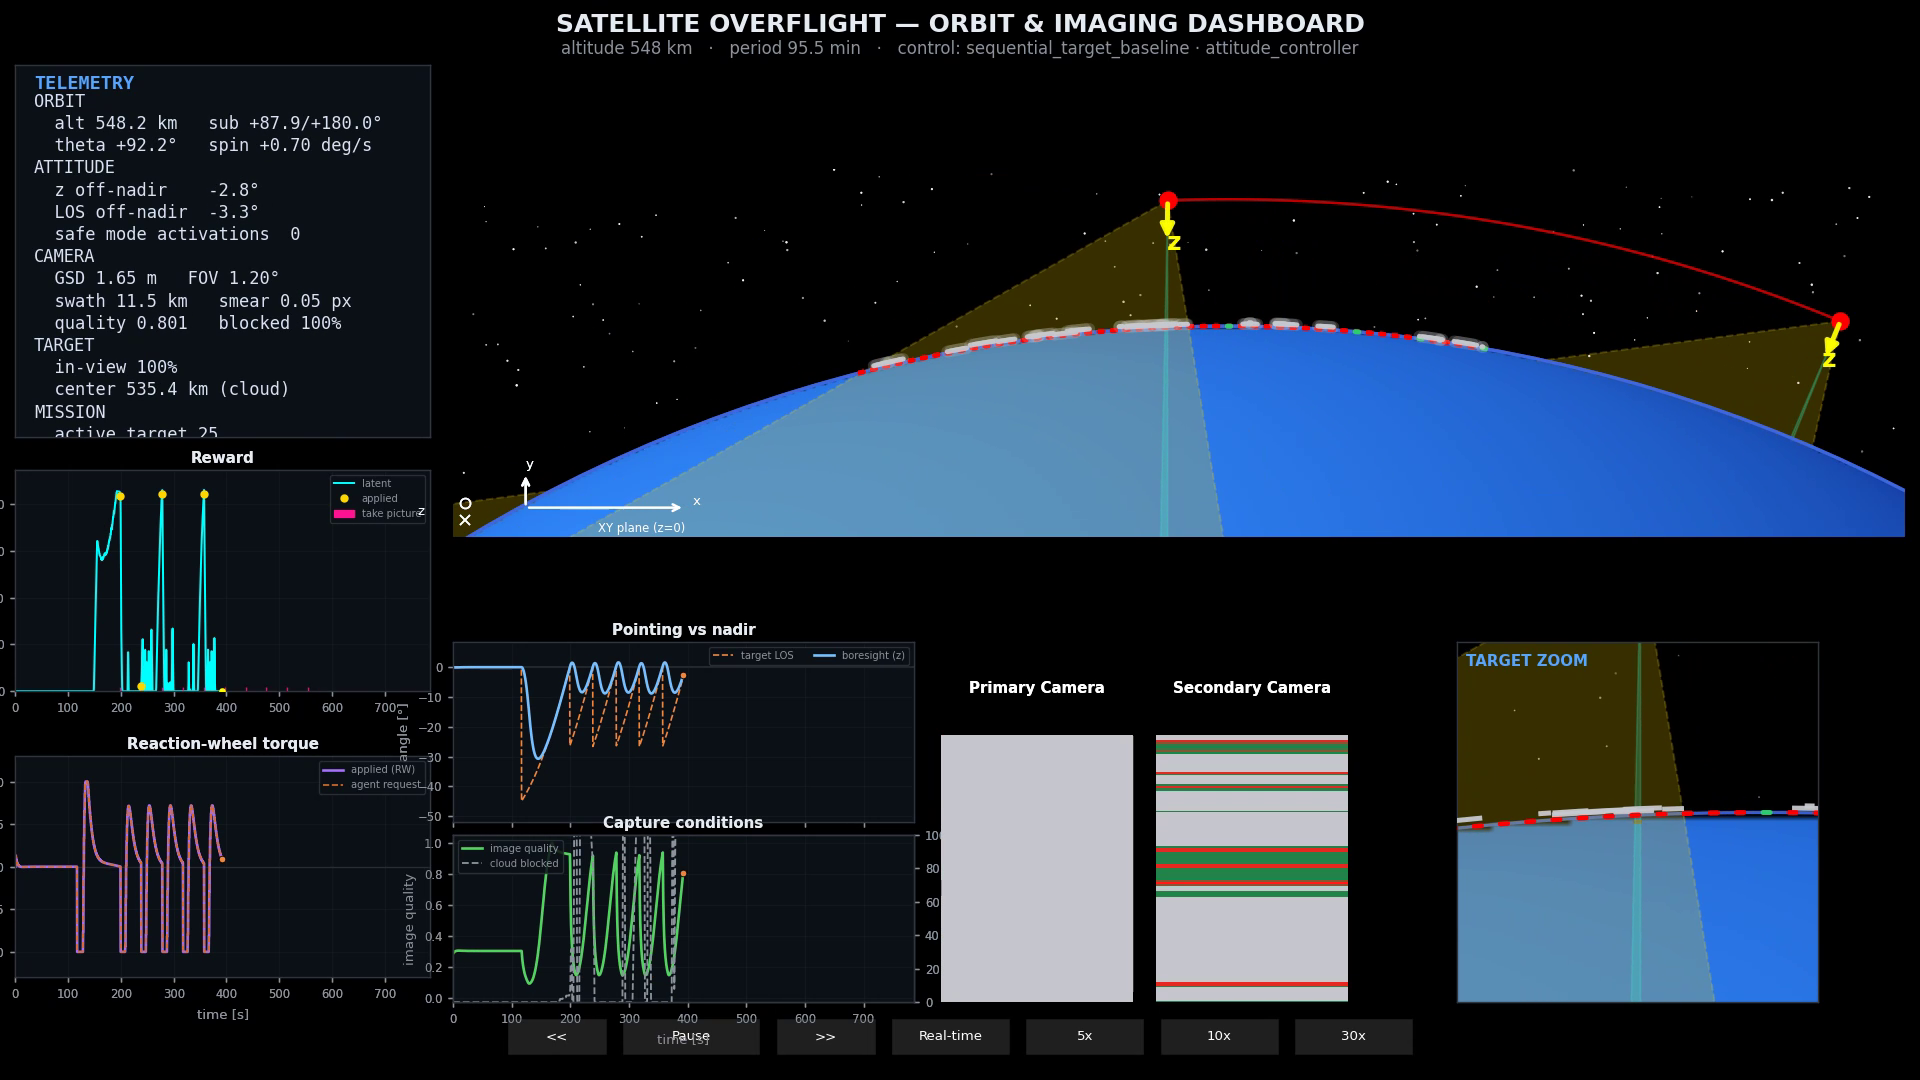
\includegraphics[width=0.92\linewidth]{figures/fig_env_overview.png}
  \caption{Environment overview on the orbit-disk dashboard early in the pass: satellite on the arc, target corridor markers on the Earth limb ahead of the boresight, before the first scheduled slew.}
  \label{fig:env-overview}
\end{figure}

\paragraph{Episode window.}
The episode start and end positions along the pass were tuned so that the first target is not yet visible in the secondary wide-angle camera at episode open, with a small margin at both boundaries.
This trims dead coast time at the corridor edges while keeping the engagement arc inside the pass.
At the canonical simulation timestep of $\Delta t = \SI{1.5}{\second}$ this yields approximately 516 controller steps per episode ($\approx\SI{774}{\second}$).

\paragraph{Off-policy learning and replay buffer.}
\label{sec:replay-buffer}
Training uses two off-policy algorithms, SAC (Section~\ref{sec:sac}) and MPO (Section~\ref{sec:mpo}): the policy is improved from stored past experience, not only from the latest rollout.
After each simulation step the transition (observation, action, reward, next observation) is appended to a \emph{replay buffer}, a fixed-capacity store of recent steps.
Gradient updates draw random mini-batches from this buffer, so a rare rewarded event (a successful capture) can contribute to many parameter updates.
\emph{Capture credit} (the reward applied when a shutter yields a useful first-time observation of a target) is sparse in this environment, so both the simulation timestep below and the warmup protocol in Section~\ref{sec:experiments} affect whether the buffer contains enough useful transitions to learn from.

\paragraph{Simulation timestep selection.}
Choosing $\Delta t$ requires balancing three competing constraints:
\begin{enumerate}
  \item \textbf{Controller authority:} $\Delta t$ must be small enough that the low-level attitude controller can still respond to the reaction-wheel dynamics within one step.
  \item \textbf{Agent decisiveness:} the agent must be able to take meaningful pointing and shutter actions on a timescale relevant to the target encounter windows.
  \item \textbf{Reward signal fidelity:} capture credit arrives only at shutter events on clear targets, so most steps carry little or no reward.
    If $\Delta t$ is too large, target encounters fall between steps and fewer rewarded transitions are stored per episode, leaving the replay buffer (Section~\ref{sec:replay-buffer}) with too little signal for off-policy learning.
\end{enumerate}
To find the largest $\Delta t$ satisfying these constraints we ran a timestep parity sweep over four candidates:
$\Delta t \in \{0.4,\,0.8,\,1.0,\,1.5\}\,\si{s}$, with controller update interval matched to $\Delta t$.
Each candidate ran one baseline warmup episode and had to satisfy: at least one shutter and episode return $\ge 50\%$ of the $\SI{0.4}{s}$ reference.
All four candidates passed.
$\Delta t = \SI{1.5}{\second}$ was selected as the largest parity-passing timestep, cutting the episode from $\sim 1935$ to $\sim 516$ controller steps and proportionally increasing training throughput.

% ─────────────────────────────────────────────────────────────────────────────
\subsection{Simplifications}
\label{sec:simplifications}

Table~\ref{tab:simplifications} summarises which subsystems are modelled and which are deliberately omitted.

\begin{table}[htbp]
  \centering
  \caption{Modelled vs.\ not-modelled subsystems.}
  \label{tab:simplifications}
  \renewcommand{\arraystretch}{1.3}
  \small
  \begin{tabular}{@{}>{\raggedright\arraybackslash}p{0.22\linewidth}>{\raggedright\arraybackslash}p{0.36\linewidth}>{\raggedright\arraybackslash}p{0.34\linewidth}@{}}
    \toprule
    Subsystem & Modelled & Not modelled \\
    \midrule
    Orbit propagation     & Circular 2D (disk model) & $J_2$, atmospheric drag, eclipse \\
    Attitude dynamics     & 2D rigid body, reaction-wheel torque chain & 3-axis, flexibility, RW friction \\
    Camera                & 1D ray tracing, image quality (motion smear) & Radiometric calibration, TDI, MTF \\
    Cloud occlusion       & Parameterised cloud-arc primitives & Spatially correlated fields, multi-layer \\
    Terrain               & Spherical Earth (WGS84 for geodesy only) & DEM, shadow, surface reflectance \\
    Multi-orbit mission   & Single pass per episode & Revisit scheduling, downlink windows \\
    Hardware latency      & Not modelled & Onboard CPU budget, comms delay \\
    \bottomrule
  \end{tabular}
\end{table}

The 2D simplification is the most consequential: all attitude variables are scalar ($\theta_\text{body}$, $\omega_\text{sat}$, $\omega_\text{wheel}$), and out-of-plane dynamics are absent.
This is consistent with the scope stated in the introduction and is a known limitation (Section~\ref{sec:limitations}).

% ─────────────────────────────────────────────────────────────────────────────
\subsection{Dynamics model}
\label{sec:dynamics}

\paragraph{Equations of motion.}
The satellite body angle $\theta_\text{b}$ and inertial rate $\omega_\text{sat}$ evolve under a single-axis reaction-wheel coupling:
\begin{align}
  \dot\omega_\text{sat} &= -\,\frac{\tau_\text{wheel}}{I_\text{sat}}, &
  \dot\omega_\text{wheel} &= \frac{\tau_\text{wheel}}{I_\text{wheel}}, &
  \dot\theta_\text{b} &= \omega_\text{sat},
\end{align}
where $I_\text{sat} = \SI{31.2}{kg.m^2}$ (Table~\ref{tab:constants-earth-spacecraft}) and
the wheel inertia $I_\text{wheel} = \tau_\text{max,RW}/\omega_\text{w,max}= \SI{0.1}{N.m}/\SI{150}{rad.s^{-1}}$.
Both are integrated forward with forward-Euler at $\Delta t_\text{sim} = \SI{1.5}{\second}$ (Table~\ref{tab:constants-camera-sim}).

\paragraph{Reaction-wheel limits.}
The wheel applies a torque $|\tau_\text{wheel}|\le\tau_\text{max,RW}=\SI{0.1}{N.m}$ and
stores angular momentum up to $H_\text{max}=\SI{0.4}{N.m.s}$.
A low-level rate gate blocks commands that would accelerate the satellite body beyond the star-tracker rate limit of $\dot\theta_\text{max}=\SI{3}{\degree.s^{-1}}$; decelerating torques are always passed.

\paragraph{Satellite mass.}
Bus mass is $m_\text{sat}=\SI{250}{kg}$ (relevant only for orbit-speed computation; inertia is the primary dynamics parameter).

% ─────────────────────────────────────────────────────────────────────────────
\subsection{Overflight and observation model}
\label{sec:obs-model}

\paragraph{Camera geometry.}
The primary nadir-looking camera parameters are listed in Table~\ref{tab:constants-camera-sim}.
The vertical field of view and ground-sampling distance (GSD) are computed analytically from sampled altitude using a pinhole model.
At $\SI{540}{km}$ the nominal GSD is approximately $\SI{1.6}{m}$.

\paragraph{Lookahead sensing.}
The secondary camera is a forward-tilted wide-angle (fisheye) imager: $\SI{25}{\degree}$ off nadir in the prograde direction with a $\SI{70}{\degree}$ along-track field of view
(Table~\ref{tab:constants-camera-sim}).
It provides early visibility of upcoming targets and cloud occlusion so the controller can decide among multiple imaging opportunities before they enter the primary nadir footprint (Section~\ref{sec:solution-concept}).

\paragraph{Camera observation lines.}
At each simulation timestep the primary and secondary cameras are evaluated as one-dimensional observation lines spanning their vertical fields of view (Table~\ref{tab:constants-camera-sim}).
Each line reports target coverage and cloud occlusion along the boresight strip; both use the same ray-intersection kernel.

\paragraph{Image quality and motion smear.}
Capturing a useful image requires the boresight ground footprint to remain nearly stationary during
the exposure window.
The full derivation proceeds in three steps: (i) compute the boresight ground velocity $v_\text{bore}$
from orbit and body rates; (ii) convert to a physical ground blur $\delta$ during exposure; (iii) map
$\delta$ to a scalar quality score $q\in[0,1]$.

\subparagraph{Step 1: Boresight ground speed.}
In the 2D orbit-disk model the satellite position is
\begin{equation}
  \vec{s} = r_\text{orb}\,[\cos\theta_\text{orb},\,\sin\theta_\text{orb}]^\top,
\end{equation}
with orbital radius $r_\text{orb}$ and true anomaly $\theta_\text{orb}(t)$ advancing at angular rate
$\dot\theta_\text{orb} = \omega_\text{orb}$.
The boresight unit vector in the disk plane is
\begin{equation}
  \hat{d} = [\cos\phi,\,\sin\phi]^\top,\qquad
  \dot\phi = \omega_\text{body},
\end{equation}
where $\phi$ is the absolute boresight angle (body angle plus nadir direction) and
$\omega_\text{body} = \dot\theta_\text{body}$ is the current body rate.

The boresight ray $\vec{s} + t\,\hat{d}$ intersects the WGS84 oblate spheroid
($a = \SI{6378137}{m}$, $b = \SI{6356752}{m}$) at slant distance $t^\star$ from the
positive root of
\begin{equation}
  A\,t^2 + B\,t + C = 0, \label{eq:ray-ellipsoid}
\end{equation}
where
\begin{align}
  A &= \frac{d_x^2 + d_y^2}{a^2} + \frac{d_z^2}{b^2}, \\
  B &= 2\!\left(\frac{s_x d_x + s_y d_y}{a^2} + \frac{s_z d_z}{b^2}\right), \\
  C &= \frac{s_x^2 + s_y^2}{a^2} + \frac{s_z^2}{b^2} - 1.
\end{align}
(All 3-D coordinates are obtained by embedding the 2D disk in the $(x,z)$ ECEF plane.)

The boresight ground hit is $\vec{g} = \vec{s} + t^\star\,\hat{d}$.
Differentiating implicitly with respect to time:
\begin{equation}
  \dot t^\star = -\,\frac{\dot A\,(t^\star)^2 + \dot B\,t^\star + \dot C}{2A\,t^\star + B},
  \label{eq:tdot}
\end{equation}
where $\dot A$, $\dot B$, $\dot C$ are computed from $\dot{\vec{s}}$ (satellite velocity) and
$\dot{\hat{d}}$ (boresight rotation rate):
\begin{equation}
  \dot{\vec{s}} = r_\text{orb}\,\omega_\text{orb}\,[-\sin\theta_\text{orb},\,0,\,\cos\theta_\text{orb}]^\top,
  \qquad
  \dot{\hat{d}} = \omega_\text{body}\,[-\sin\phi,\,0,\,\cos\phi]^\top.
\end{equation}
The hit velocity is then
\begin{equation}
  \dot{\vec{g}} = \dot{\vec{s}} + \dot t^\star\,\hat{d} + t^\star\,\dot{\hat{d}}.
  \label{eq:gdot}
\end{equation}
The boresight ground speed is $v_\text{bore} = \|\dot{\vec{g}}\|$.

\subparagraph{Step 2: Ground blur during exposure.}
During a finite exposure $t_\text{exp} = \SI{100}{\micro s}$ the boresight footprint moves
\begin{equation}
  \delta = v_\text{bore}\,t_\text{exp}\quad[\si{m}].
\end{equation}
The pixel smear in GSD units is
\begin{equation}
  \sigma = \frac{\delta}{\text{GSD}_\text{eff}},
\end{equation}
where the effective GSD at off-nadir angle $\alpha$ is
$\text{GSD}_\text{eff} = \text{GSD}_0 / \cos\alpha$,
with nadir GSD
\begin{equation}
  \text{GSD}_0 = \frac{p\cdot h}{f} = \frac{\SI{3.2}{\micro m}\cdot h}{\SI{1067}{mm}}
\end{equation}
(pixel pitch $p$, altitude $h$, focal length $f$).
At $h = \SI{540}{km}$: $\text{GSD}_0 \approx \SI{1.62}{m}$,
giving a nadir swath of $9344 \times \SI{1.62}{m} \approx \SI{15.1}{km}$ along-track.

\subparagraph{Step 3: Normalised quality score.}
Rather than using smear in pixels (which depends on altitude), quality is expressed in physical
ground units via a Lorentzian:
\begin{equation}
  q = \frac{r}{\delta + r}, \qquad
  r = \SI{0.30}{m},\quad t_\text{exp} = \SI{100}{\micro s}.
  \label{eq:quality}
\end{equation}
Properties: $q \to 1$ as $\delta \to 0$ (perfect tracking); $q = 0.5$ at $\delta = r = \SI{0.30}{m}$;
$q$ is indifferent to GSD (quality degrades from optical smear, not pixel count).

\subparagraph{Characteristic regimes.}
At the canonical orbit ($h = \SI{540}{km}$, $\omega_\text{orb} \approx \SI{1.08e-3}{rad.s^{-1}}$):
\begin{itemize}
  \item \textbf{Nadir, zero body rate:} $v_\text{bore} = r_\text{orb}\,\omega_\text{orb} \approx \SI{7.6}{km.s^{-1}}$,
    $\delta \approx \SI{0.76}{m}$, $q \approx 0.28$.
  \item \textbf{Target-tracking ($\omega_\text{body} = \omega_\text{orb}$):} $v_\text{bore} \approx 0$,
    $\delta \approx 0$, $q \approx 1.0$.
  \item \textbf{Half-tracking:} $\omega_\text{body} = 0.5\,\omega_\text{orb}$,
    $\delta \approx \SI{0.38}{m}$, $q \approx 0.44$.
\end{itemize}
The quality factor directly enters the capture-credit reward (Eq.~\ref{eq:r-cap}),
giving the agent an incentive to slow the boresight ground motion by pointing toward
and tracking each target across its observation window.

\begin{figure}[htbp]
  \centering
  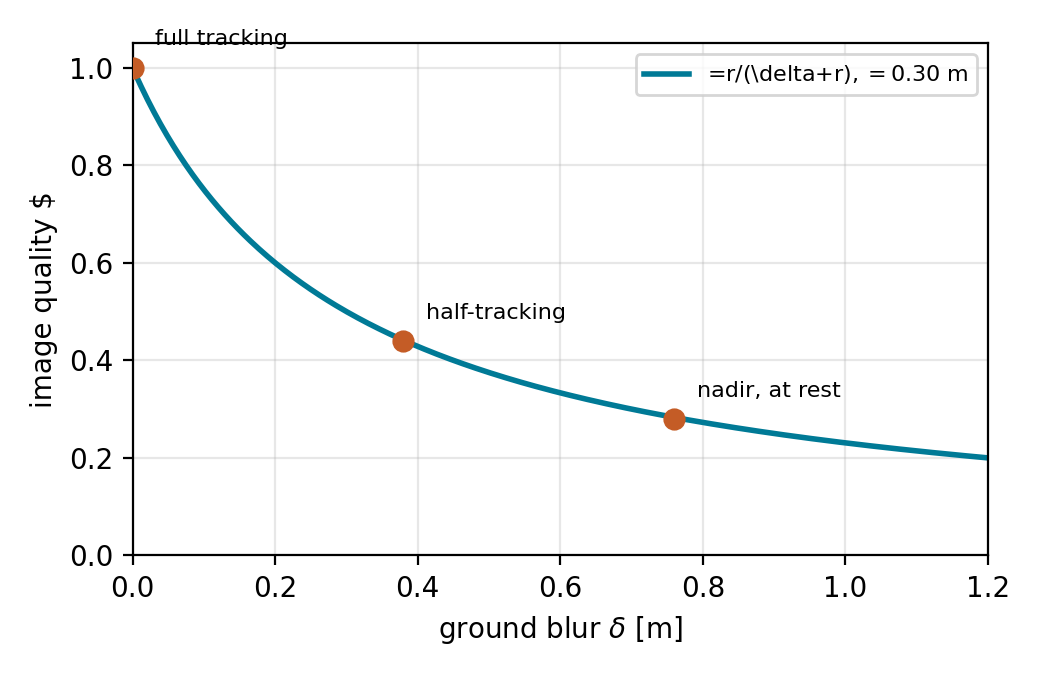
\includegraphics[width=0.72\linewidth]{figures/fig_image_quality_curve.png}
  \caption{Normalised image quality $q=r/(\delta+r)$ with $r=\SI{0.30}{m}$.
    Annotated operating points match the nadir-at-rest, half-tracking, and full-tracking regimes above.}
  \label{fig:image-quality-curve}
\end{figure}

\paragraph{Cloud model.}
Cloud primitives are parameterised arcs in the orbit plane.
For each episode a seeded generator places cloud patches along the target corridor with extent, altitude, and thickness drawn from the ranges in Table~\ref{tab:constants-mission}.
Over a single pass the clouds are effectively fixed relative to the ground corridor (any advective drift is negligible on the episode timescale); occlusion changes mainly because the satellite and camera rays move through that layout.
The cloud-blocked fraction along each camera observation line is computed at every timestep and contributed to the per-step observation and reward.

% ─────────────────────────────────────────────────────────────────────────────
\subsection{Baseline strategy}
\label{sec:baseline}

The reference controller is a deterministic sequential-target overflight policy.
Figure~\ref{fig:baseline-overflight-phases} shows the approach, point, and capture phases of a typical pass; Table~\ref{tab:baseline-config} lists the scheduling logic, OBC PD gains, lock threshold, lead margin, shutter commands, and cloud awareness.
The baseline uses the same attitude-safety stack and simulation kernel as the learned policy: safety overrides are not disabled.

\begin{table}[htbp]
  \centering
  \renewcommand{\arraystretch}{1.3}
  \caption{Deterministic baseline configuration (comparison anchor).}
  \label{tab:baseline-config}
  \small
  \begin{tabular}{p{0.32\linewidth}p{0.62\linewidth}}
    \toprule
    Aspect & Setting \\
    \midrule
    Scheduling logic &
      Strided target list: 10 captures per pass from a 50-target corridor (indices 0, 5, 10, \ldots, 45 on the evaluation seed).
      Nadir coast between engages; slew to target bearing when the orbit-angle window opens. \\
    OBC pointing &
      PD loop on body-angle tracking error; gains $k_p \approx \SI{1.15}{N.m/rad}$, $k_d \approx \SI{12.0}{N.m.s/rad}$
      derived from $\tau_\text{max}=\SI{0.1}{N.m}$, $I_\text{sat}=\SI{31.2}{kg.m^2}$, and a \SI{5}{\degree} deceleration band. \\
    Boresight lock threshold &
      $\SI{15}{\degree}$ between body boresight and target bearing (shutter fires once locked, or if image quality $\ge 0.25$ while the target is in the sensor strip). \\
    Lead margin &
      \SI{20}{\degree} orbit-angle margin before target engage window opens. \\
    Shutter commands &
      10 per episode (one per scheduled target; matches the episode capture cap). \\
    Cloud awareness &
      None (captures on schedule regardless of occlusion). \\
    \bottomrule
  \end{tabular}
\end{table}

In each learning run the same baseline policy fills five warmup episodes under that run's action interface and reward stack;
the mean warmup return is therefore the matched \emph{average baseline return} against which training and evaluation are compared (Section~\ref{sec:exp-table}).

% ─────────────────────────────────────────────────────────────────────────────
\subsection{Attitude safety controller}
\label{sec:safety}

Every torque command, whether from the learned policy or the baseline, passes through the
attitude safety controller before reaching the reaction-wheel plant.
The controller operates in two regimes:

\paragraph{Normal-mode taper.}
In nominal flight the controller applies a linear taper on the commanded torque when the satellite approaches the off-nadir hard limit:
\begin{equation}
  \tau_\text{applied} = \alpha\,\tau_\text{cmd}, \qquad
  \alpha = \mathrm{clip}\!\left(\frac{\theta_\text{hard} - \theta_\text{off-nadir}}{\theta_\text{hard} - \theta_\text{arm}},\,0,\,1\right),
\end{equation}
where $\theta_\text{hard}=\SI{45}{\degree}$ is the hard limit and $\theta_\text{arm}$ is the kinematic braking distance
($\theta_\text{arm}=\theta_\text{hard} - \omega^2/(2\tau_\text{max}/I_\text{sat})$).

\paragraph{Safe-mode entry condition.}
Safe mode is entered when the off-nadir angle equals or exceeds $\theta_\text{hard}$, or when the predicted
overshoot satisfies $\theta_\text{off-nadir} + \theta_\text{brake} \ge \theta_\text{hard}$.

\paragraph{Safe-mode recovery phases.}
Once safe mode is active the agent torque command is replaced by an onboard recovery sequence
(agent commands are ignored throughout):
\begin{enumerate}
  \item \textbf{BRAKE:} zero-rate command until $|\omega_\text{sat}-\omega_\text{orbit}|\le\SI{0.1}{\degree.s^{-1}}$.
  \item \textbf{CRUISE:} slew toward nadir at $\pm\SI{0.35}{\degree.s^{-1}}$ until off-nadir $\le\SI{5.0}{\degree}$.
  \item \textbf{SETTLE:} zero-rate command until off-nadir $\le\SI{1.0}{\degree}$ and rate $\le\SI{0.1}{\degree.s^{-1}}$.
  \item \textbf{LOCKOUT:} hold nadir for $\SI{60}{s}$; agent torque rejected.
\end{enumerate}
After LOCKOUT the controller exits safe mode and normal operation resumes.
All phase thresholds are listed in Table~\ref{tab:safety-thresholds}.

\begin{figure}[htbp]
  \centering
  \begin{subfigure}[t]{0.32\linewidth}
    \centering
    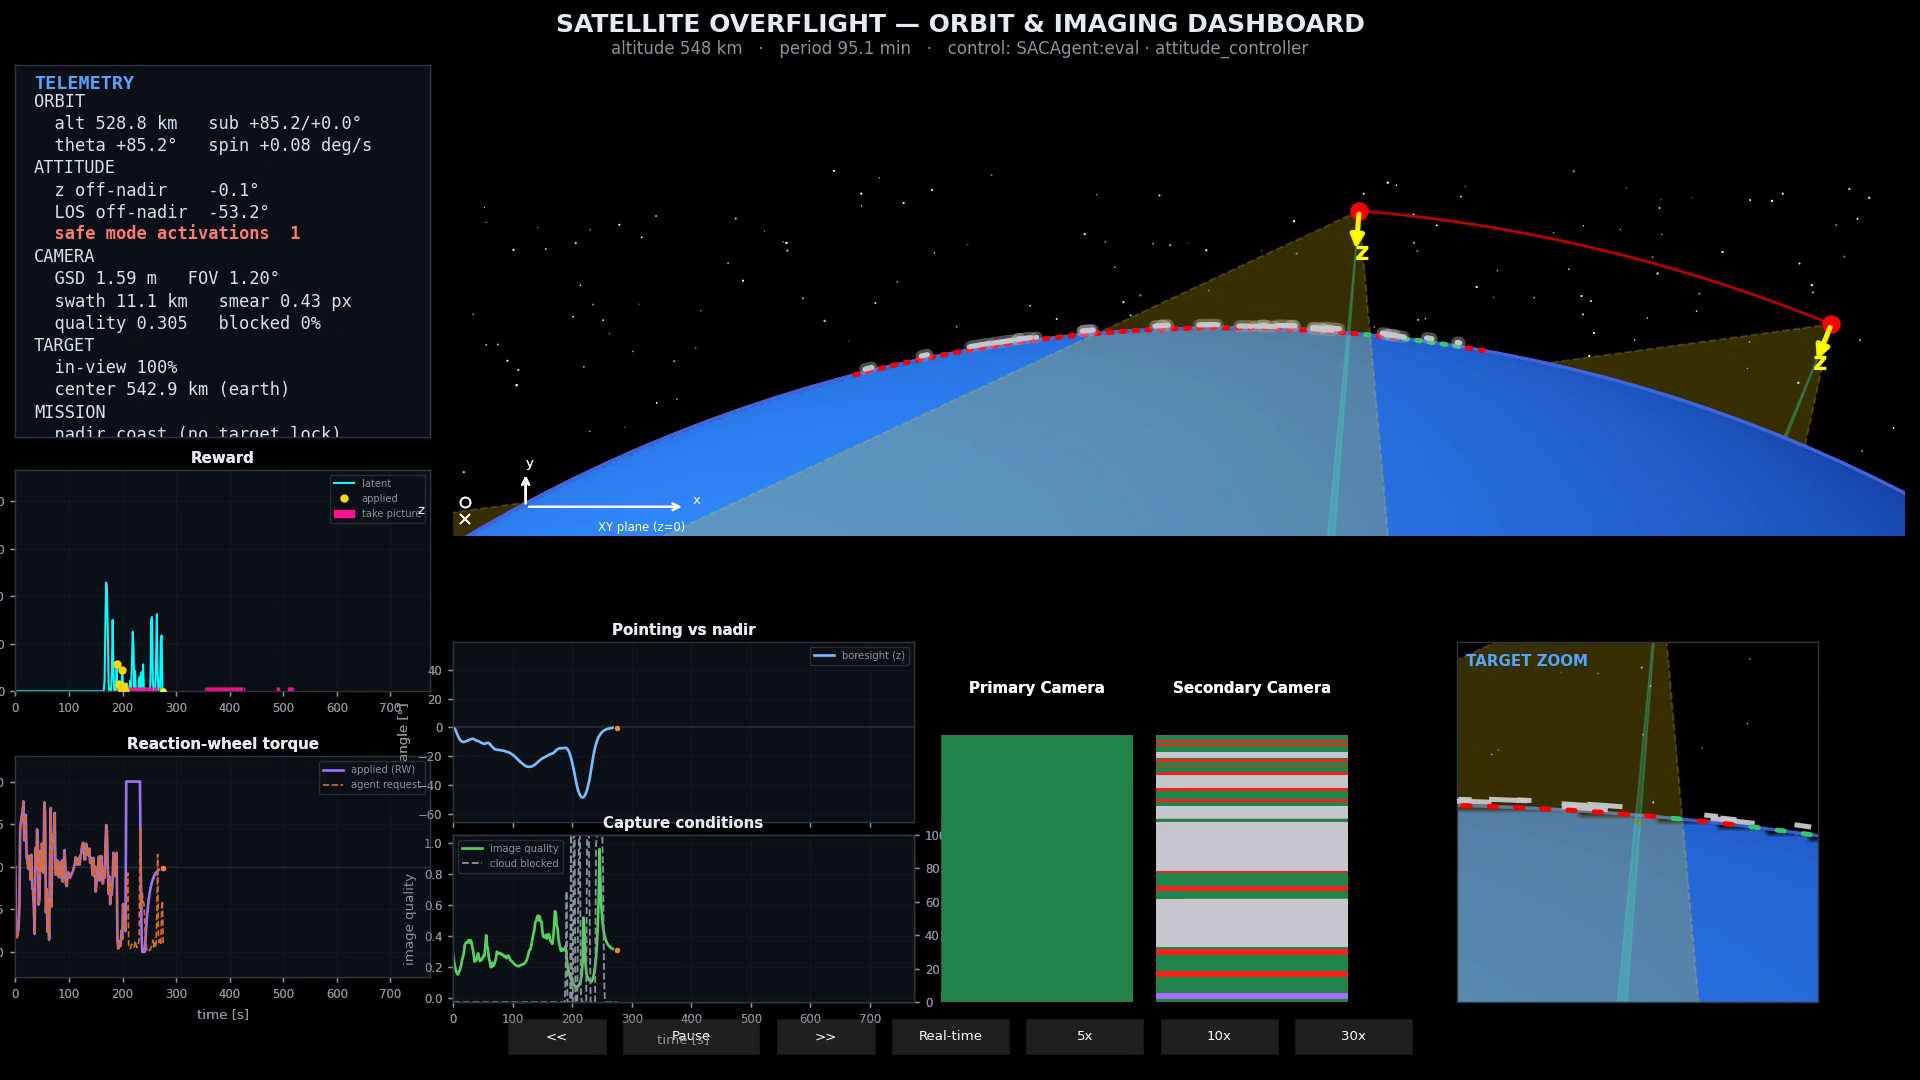
\includegraphics[width=\linewidth]{figures/fig_safety_t0.png}
    \caption{High-torque slew (BRAKE)}
  \end{subfigure}\hfill
  \begin{subfigure}[t]{0.32\linewidth}
    \centering
    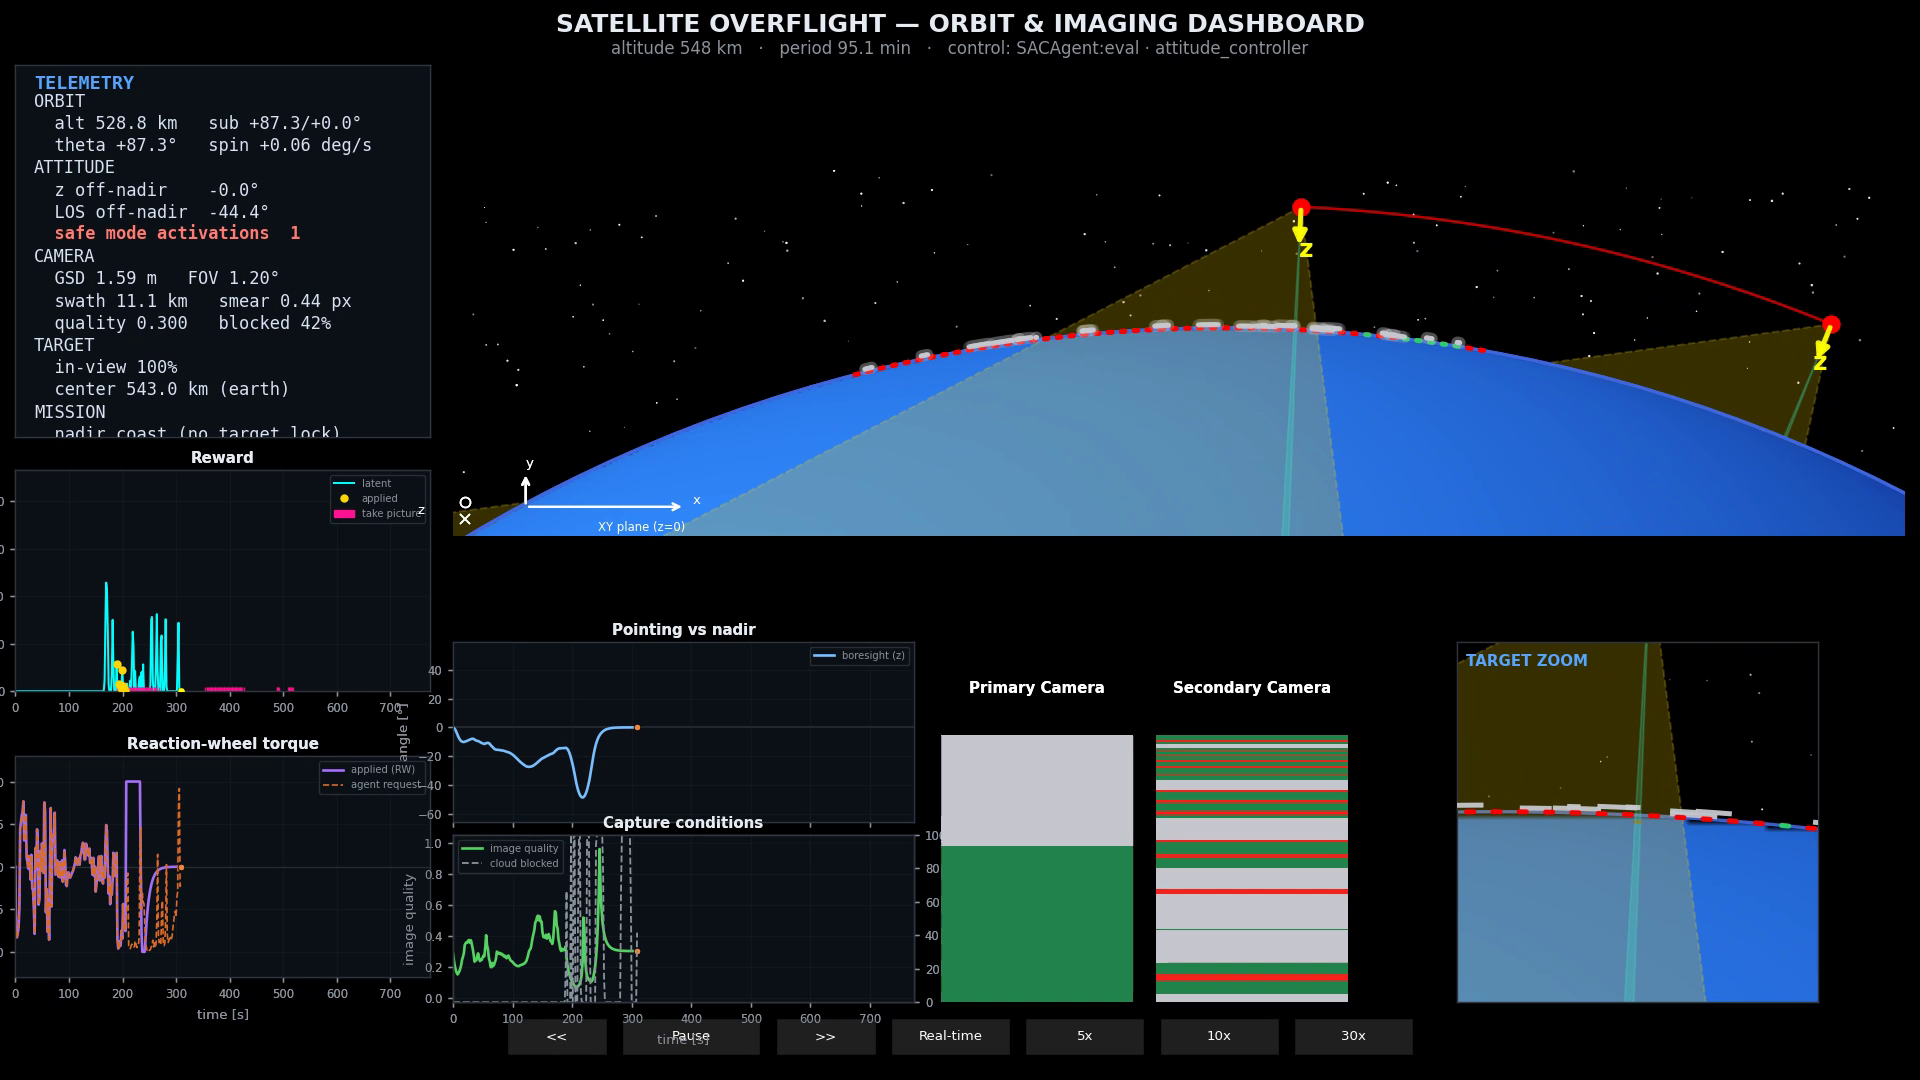
\includegraphics[width=\linewidth]{figures/fig_safety_t1.png}
    \caption{CRUISE}
  \end{subfigure}\hfill
  \begin{subfigure}[t]{0.32\linewidth}
    \centering
    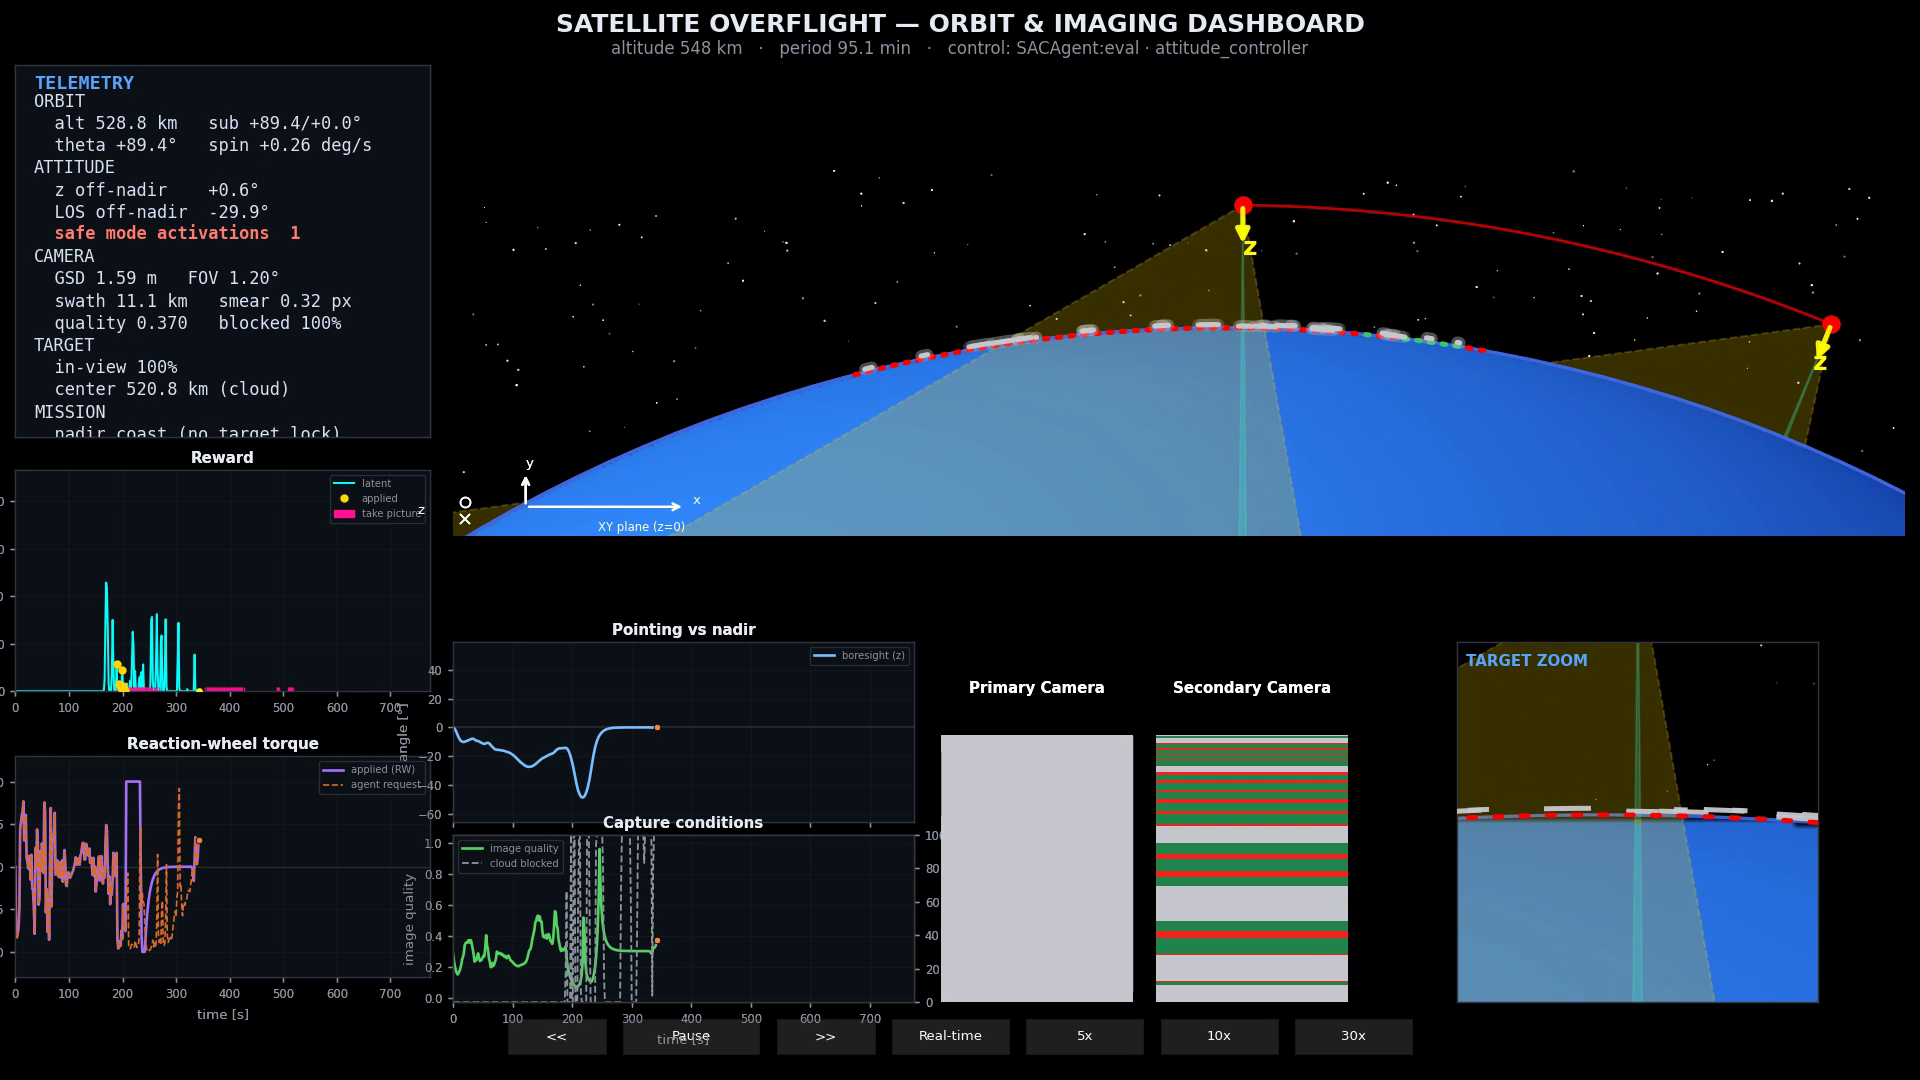
\includegraphics[width=\linewidth]{figures/fig_safety_t2.png}
    \caption{LOCKOUT}
  \end{subfigure}
  \caption{One attitude-safety cycle in torque-mode evaluation (same episode; panels use the recovery-phase names BRAKE / CRUISE / LOCKOUT).
    (a)~High-torque slew: the agent commands large torque and reaches $\approx\SI{43}{\degree}$ off-nadir; safe mode activates (BRAKE) and rejects the request (applied torque drops while the agent request remains high).
    (b)~CRUISE: onboard recovery slews the boresight back toward nadir (here $\approx\SI{24}{\degree}$ off-nadir) while agent torque stays ignored.
    (c)~LOCKOUT: nadir hold with agent torque rejected for $\SI{60}{s}$.
    SETTLE (between CRUISE and LOCKOUT) is short and not shown.}
  \label{fig:safety-maneuver}
\end{figure}

\begin{table}[htbp]
  \centering
  \caption{Attitude safety controller thresholds.}
  \label{tab:safety-thresholds}
  \begin{tabular}{lll}
    \toprule
    Parameter & Symbol & Value \\
    \midrule
    Off-nadir hard limit          & $\theta_\text{hard}$     & $\SI{45}{\degree}$ \\
    Nadir recovery tolerance      & $\theta_\text{tol}$      & $\SI{1.0}{\degree}$ \\
    Decel start (CRUISE$\to$SETTLE) & $\theta_\text{decel}$  & $\SI{5.0}{\degree}$ \\
    Rate stop threshold           & $\omega_\text{stop}$     & $\SI{0.1}{\degree.s^{-1}}$ \\
    Safe-mode cruise rate         & $\dot\theta_\text{crs}$  & $\SI{0.35}{\degree.s^{-1}}$ \\
    Post-recovery lockout         & $t_\text{lock}$          & $\SI{60}{s}$ \\
    \bottomrule
  \end{tabular}
\end{table}

% ─────────────────────────────────────────────────────────────────────────────
\subsection{Reward design}
\label{sec:reward}

The reward is computed per controller step from the full episode simulation state.
All active terms are listed below; inactive terms (distance reward, cloud penalty, energy penalty) were tested in early experiments and disabled by default (see Section~\ref{sec:experiments}).

\paragraph{Capture quality term (applied at shutter events).}
When the agent fires the shutter, is within budget, and the target has not been captured before:
\begin{equation}
  r_\text{cap} = W_\text{cap}\cdot\text{cov}\cdot q\cdot(1 - f_\text{cloud}),
  \label{eq:r-cap}
\end{equation}
where $\text{cov}\in[0,1]$ is the fraction of the primary camera footprint over the dominant target,
$q\in[0,1]$ is the image quality (Section~\ref{sec:obs-model}),
$f_\text{cloud}\in[0,1]$ is the cloud-blocked fraction, and
$W_\text{cap}$ is the capture weight.
Repeat shutters on an already-captured target consume budget but yield zero applied reward.

\paragraph{Budget-exhausted penalty.}
When the agent commands a shutter after the 10-capture budget is exhausted:
$r_\text{budget} = -k_\text{waste}$ with $k_\text{waste}=5.0$ (Exp~7, promoted to default).

\paragraph{Shutter-waste penalty (off by default).}
Optional: when applied capture credit $< \epsilon = 0.001$ on an accepted shutter:
$r_\text{waste} = -k_\text{waste}$. Removed in Exp~9 (see Section~\ref{sec:exp9}).

\paragraph{Torque-effort regulariser (torque mode only).}
\begin{equation}
  r_\text{effort} = -k_\text{eff}\left(\frac{\tau_\text{cmd}}{\tau_\text{max}}\right)^2,
  \qquad k_\text{eff}=0.1.
\end{equation}
Applied every step on the agent-requested torque (before safety arbitration); disabled automatically in vector mode.

\paragraph{Safe-mode penalty (Exp~10 only, not default).}
Per-step penalty while the agent is in safe-mode recovery: $r_\text{safe} = -k_\text{safe}$, $k_\text{safe}=2.0$.
Ruled out at this coefficient (see Section~\ref{sec:exp10}).

% ─────────────────────────────────────────────────────────────────────────────
\subsection{Learning algorithm: SAC}
\label{sec:sac}

We use Soft Actor-Critic (SAC) \cite{haarnoja2018sac}.
SAC is an off-policy actor-critic algorithm in the \emph{maximum-entropy} reinforcement-learning framework:
the stochastic policy maximises expected return while also maximising action entropy, so that high-reward behaviour is learned without collapsing prematurely to a near-deterministic action.
In continuous control, this yields a stable off-policy learner that reuses replay-buffer experience and explores via the entropy term rather than via an additive noise process.

\paragraph{Soft critic update (policy evaluation).}
Two critics $Q_{\theta_1},Q_{\theta_2}$ are trained against a shared soft Bellman target built from the minimum of the target critics (clipped double-Q), with an entropy bonus on the next action:
\begin{equation}
  y = r + \gamma(1-d)\,
  \Bigl(
    \min_{i\in\{1,2\}} Q_{\theta_i'}(s',a')
    - \alpha\,\log\pi_\phi(a'|s')
  \Bigr),
  \label{eq:sac-soft-bellman}
\end{equation}
where $a'\sim\pi_\phi(\cdot|s')$, $d\in\{0,1\}$ marks episode termination, and target networks $Q_{\theta_i'}$ are soft-updated with coefficient $\tau$ (Table~\ref{tab:sac-hparams}).
Each critic is fitted by mean-squared error to $y$.

\paragraph{Policy update (soft actor).}
The Gaussian actor $\pi_\phi$ is updated to maximise soft $Q$ while retaining entropy:
\begin{equation}
  J_\pi(\phi)
  = \mathbb{E}_{s\sim\mathcal{B},\,a\sim\pi_\phi}\!
  \Bigl[
    \alpha\,\log\pi_\phi(a|s)
    - \min_{i\in\{1,2\}} Q_{\theta_i}(s,a)
  \Bigr],
  \label{eq:sac-policy}
\end{equation}
which is minimised by stochastic gradient descent (reparameterised samples; tanh-squashed actions with the standard change-of-variables correction on $\log\pi$).

\paragraph{Fixed entropy temperature.}
The temperature $\alpha$ trades off return against entropy.
We use a fixed coefficient $\alpha=0.2$ (no automatic temperature dual), matching the overnight SAC fork used throughout the experiment series.
This is simpler than the learned-$\alpha$ variant of SAC and was sufficient for the sparse-reward regimes in which SAC first showed a learning signal (Exp~3).

\paragraph{Network architecture.}
Actor and critics use the same 1D-CNN encoder and fully connected widths as MPO (Section~\ref{sec:mpo}): two convolutional layers (kernel size~5, channels $[16,32]$, stride~2, embedding dimension~32), then actor head 90 units and critic heads 140 units.
Hyperparameters are listed in Table~\ref{tab:sac-hparams}.

\begin{table}[htbp]
  \centering
  \caption{SAC hyperparameters (default configuration; all SAC experiments unless noted).}
  \label{tab:sac-hparams}
  \begin{tabular}{lll}
    \toprule
    Parameter & Symbol & Value \\
    \midrule
    Batch size               & $B$               & 256 \\
    Replay buffer            & $|\mathcal{B}|$   & 50\,000 \\
    Discount factor          & $\gamma$          & 0.99 \\
    Target network           & $\tau$            & 0.005 \\
    Actor learning rate      & $\eta_\pi$        & $1.5\times10^{-4}$ \\
    Critic learning rate     & $\eta_Q$          & $4.5\times10^{-4}$ \\
    Entropy temperature      & $\alpha$          & 0.2 (fixed) \\
    Warmup episodes           & ---               & 5 \\
    Training episodes         & ---               & 50 (Exp~2: 7) \\
    Eval episodes             & ---               & 2 \\
    Environment seed          & ---               & 7 \\
    \bottomrule
  \end{tabular}
\end{table}

% ─────────────────────────────────────────────────────────────────────────────
\subsection{Learning algorithm: MPO}
\label{sec:mpo}

We use Maximum a Posteriori Policy Optimisation (MPO) \cite{abdolmaleki2018mpo}.
MPO frames policy improvement as a constrained relative-entropy problem solved by alternating E-step and M-step:

\paragraph{E-step (sample-based policy evaluation).}
$Q^\pi$ targets are regressed from a target critic; the new non-parametric policy distribution
$q^\star(a|s) \propto \pi(a|s)\exp(Q^\pi(s,a)/\eta)$
is derived by solving the dual:
\begin{equation}
  \eta^\star = \arg\min_{\eta>0}\;\eta\,\varepsilon_\eta + \eta\log\mathbb{E}_{\pi}\!\left[\exp\!\left(\frac{Q^\pi(s,a)}{\eta}\right)\right],
  \label{eq:mpo-dual}
\end{equation}
where $\varepsilon_\eta=0.1$ is the KL constraint on the temperature dual.

\paragraph{M-step (policy update with trust region).}
A parametric Gaussian policy $\pi_\theta$ is fitted to $q^\star$ subject to decoupled KL constraints on the mean and variance:
\begin{equation}
  \max_\theta\;\mathbb{E}_{q^\star}\!\left[\log\pi_\theta(a|s)\right]
  \quad\text{s.t.}\quad
  \mathrm{KL}(\bar\pi_\mu\|\pi_{\theta,\mu})\le\varepsilon_\mu,\;
  \mathrm{KL}(\bar\pi_\sigma\|\pi_{\theta,\sigma})\le\varepsilon_\sigma,
\end{equation}
with Lagrange multipliers $\alpha_\mu,\alpha_\sigma$ updated by dual ascent
($\varepsilon_\mu=0.1$, $\varepsilon_\sigma=0.01$; Table~\ref{tab:mpo-hparams}).

\paragraph{Decoupled-KL fix (Exp~8).}
Prior to Exp~8 the implementation used a single coupled KL constraint with a shared multiplier,
which led to KL $\to 0$ (frozen policy) or KL $\to \infty$ (exploding critic) depending on initialisation.
The fix implements separate $\alpha_\mu/\alpha_\sigma$ multipliers as specified in \citet{abdolmaleki2018mpo}.
All MPO experiments from Exp~8 onwards use the corrected implementation.

\paragraph{Network architecture.}
Both actor and critic share a 1D-CNN encoder over the camera observation lines (two convolutional layers, kernel size~5, channels $[16,32]$, stride~2, embedding dimension~32)
followed by fully connected layers (actor: 90 units; critic: 140 units).
Hyperparameters are listed in Table~\ref{tab:mpo-hparams}.

\begin{table}[htbp]
  \centering
  \caption{MPO hyperparameters (default configuration; all experiments unless noted).}
  \label{tab:mpo-hparams}
  \begin{tabular}{lll}
    \toprule
    Parameter & Symbol & Value \\
    \midrule
    Batch size               & $B$               & 256 \\
    Replay buffer            & $|\mathcal{B}|$   & 50\,000 \\
    Discount factor          & $\gamma$          & 0.99 \\
    Target network           & $\tau$            & 0.005 \\
    Actor learning rate      & $\eta_\pi$        & $4.5\times10^{-4}$ \\
    Critic learning rate     & $\eta_Q$          & $1.0\times10^{-3}$ \\
    Dual learning rate       & $\eta_\eta$       & $1.0\times10^{-3}$ \\
    KL samples (E-step Q)    & $N_Q$             & 80 \\
    KL samples (M-step)      & $N_\pi$           & 40 \\
    KL temperature constraint & $\varepsilon_\eta$ & 0.1 \\
    KL mean constraint        & $\varepsilon_\mu$  & 0.1 \\
    KL variance constraint    & $\varepsilon_\sigma$& 0.01 \\
    Warmup episodes           & ---               & 5 \\
    Training episodes         & ---               & 50 (except Exp~14: 350) \\
    Eval episodes             & ---               & 2 \\
    Environment seed          & ---               & 7 (Exps~1--13) \\
    \bottomrule
  \end{tabular}
\end{table}

% ─────────────────────────────────────────────────────────────────────────────
\subsection{Observation and action space}
\label{sec:obs-action}

\paragraph{Observations.}
The controller observation is assembled at each controller tick from:
\begin{itemize}
  \item \textbf{Attitude scalars:} body angle $\theta_\text{body}$ [rad], satellite body rate $\omega_\text{sat}$ [rad/s].
  \item \textbf{Orbit scalar:} true anomaly $\theta_\text{orbit}$ [rad].
  \item \textbf{Camera lines:} primary and secondary observation-line arrays (per-cell class labels: background, target identity, or cloud-blocked).
  \item \textbf{Mission context:} remaining shutter budget (dimensionless count); binary target-captured mask (one entry per target area); signed bearing error toward each target [rad].
\end{itemize}

\paragraph{Actions.}
Both SAC and MPO policies output a 2-dimensional continuous action $[a_\tau, a_s]\in[-1,1]^2$:
\begin{itemize}
  \item \textbf{Torque mode:} $a_\tau\mapsto\tau_\text{cmd} = a_\tau\cdot\tau_\text{max}$ [\si{N.m}] (direct RW torque request).
  \item \textbf{Vector mode:} $a_\tau\mapsto f_n = \SI{45}{\degree}\cdot a_\tau$ (nadir-relative pointing offset); the OBC PD controller converts this to a torque command.
  \item \textbf{Shutter:} $a_s\mapsto (a_s+1)/2\in[0,1]$; boolean shutter command when mapped value $> 0.5$.
\end{itemize}
The torque versus vector mode is a configuration choice at training time;
experiments from Exp~11 onward use vector mode as the default.

% ─────────────────────────────────────────────────────────────────────────────
\subsection{Simulation architecture}
\label{sec:arch}

Training, evaluation, and visualisation share one simulated episode per roll-out.
The reward, the evaluation KPIs, and the exported videos therefore reflect the same altitude, cloud layout, attitude trajectory, and camera observations.
Mission randomisation is controlled by a fixed integer seed so that the deterministic baseline and each learned configuration are compared under identical environment draws.


\section{Experiments}
\label{sec:experiments}

Fourteen experiments were conducted between 2026-06-28 and 2026-07-02 to map the reward and action-space design required for cloud-aware autonomous pointing.
Each run tests one concrete design choice; the sequence is cumulative rather than a search for a single winning configuration.
The arc divides into three phases: (i) diagnosing why naive training setups fail (Exps~1--5),
(ii) reward shaping and action-space design (Exps~4--9), and
(iii) MPO-specific stabilisation and further ablations (Exps~8--12), followed by scale and cadence probes (Exps~13--14).
Experiment~6 (modular encoder rerun) was deferred and is not included.

\paragraph{Experimental protocol.}
\label{sec:exp-protocol}
A fixed random seed (7) ensures identical altitude draws, cloud layouts, and target positions across all compared runs.
All experiments share the canonical simulation architecture described in Section~\ref{sec:arch}.

Before training begins, \emph{warmup episodes} pre-fill the replay buffer (Section~\ref{sec:replay-buffer}) using the deterministic baseline policy.
This was not the initial choice: early attempts using random torque commands or a zero-torque coast strategy yielded no reward signal, because neither strategy ever issues capture commands that earn positive credit.
The baseline policy, by contrast, reliably captures targets on clear passes.
Even so, only around ten capture actions fall within a 516-step episode ($\approx 2\%$ of all transitions), so the buffer is extremely sparse in rewarded transitions.
The warmup data therefore serves a dual purpose: it bootstraps the replay buffer with at least some positive-credit transitions, and the episode return it achieves is the KPI comparison anchor used throughout.

\emph{Evaluation episodes} run the current learned policy without gradient updates; eval return is the primary metric.
A run is said to show a \emph{learning signal} if its per-episode training return trends upward over training, indicating the policy has discovered the reward structure.
Concretely, this requires at least one training episode to substantially exceed the warmup return and for the trend to be sustained rather than a single outlier.
Runs without a learning signal converge to a flat return plateau from episode~1 onward, regardless of the number of training episodes, and are reported as \emph{not supported}.
In the verdict column, \emph{supported} means the design choice under test produced the expected learning or behavioural change (for example selective shuttering or a stable upward return trend); it does not by itself claim mission-ready outperformance of the baseline.
Results are archived as JSON files per experiment; key metrics are cited directly below.

% ─────────────────────────────────────────────────────────────────────────────
\subsection{Master comparison table}
\label{sec:exp-table}

Table~\ref{tab:exp-comparison} lists the full configuration and primary KPI for every run.
The \textbf{baseline anchor} row is the deterministic baseline evaluated at matched seeds (mean eval return $-38.6$; anchored in Exp~13).

\begin{table}[htbp]
  \centering
  \caption{Master experiment comparison. Algorithm: SAC = Soft Actor--Critic; MPO = Maximum a Posteriori Policy Optimisation.
    Action: T = torque (direct RW), V = vector pointing (nadir-relative offset).
    Reward flags: B = budget-exhausted shutter penalty; W = within-budget waste penalty; E = torque effort;
    S = safe-mode per-step penalty.
    Seeds: fixed 7 for all ML experiments; env draws are seeded per warmup fingerprint.
    Eval return is mean over 2 evaluation episodes unless otherwise noted.
    $\Delta$ is relative to the immediate predecessor configuration.}
  \label{tab:exp-comparison}
  \scriptsize
  \setlength{\tabcolsep}{4pt}
  \begin{tabular}{lllllccccc}
    \toprule
    Exp & Config & Alg & Act & Reward flags & Warmup & Train & Eval eps & Eval return & Verdict \\
    \midrule
    nb07      & baseline           & ---  & V  & ---        & ---  & ---  & 2 & $-38.6$   & --- \\
    \midrule
    1         & mpo\_t05           & MPO  & T  & ---        & 5    & 7    & 2 & $-101.6$  & not\_supported \\
    1         & mpo\_t09           & MPO  & T  & ---        & 5    & 7    & 2 & $-101.6$  & not\_supported \\
    2         & sac\_a0            & SAC  & T  & ---        & 5    & 7    & 2 & $-78.9$   & not\_supported \\
    2         & sac\_a1            & SAC  & T  & ---        & 5    & 7    & 2 & $-86.5$   & not\_supported \\
    3         & compare\_sac       & SAC  & T  & ---        & 5    & 37$^\dagger$  & 2 & $-22.2$   & supported \\
    3         & compare\_mpo       & MPO  & T  & dense      & 5    & 22$^\dagger$  & 2 & $-51.6$   & not\_supported \\
    4         & ref0 (torque)      & SAC  & T  & ---        & 5    & 50   & 2 & $-11.1$   & partial \\
    4         & ref1 (vector)      & SAC  & V  & ---        & 5    & 50   & 2 & $-24.1$   & partial \\
    5         & mpo\_s (90/140)    & MPO  & T  & sparse     & 5    & 50   & 2 & $-51.6$   & not\_supported \\
    5         & mpo\_m (140/256)   & MPO  & T  & sparse     & 5    & 50   & 2 & $-51.6$   & not\_supported \\
    5         & mpo\_l (256/512)   & MPO  & T  & sparse     & 5    & 50   & 2 & $-51.6$   & not\_supported \\
    7         & penalty\_on        & SAC  & V  & B          & 5    & 50   & 2 & $+10.6$   & supported \\
    8         & torque\_sparse     & MPO* & T  & ---        & 5    & 50   & 2 & $-81.1$   & partial \\
    9         & waste\_off\_budget\_on & SAC & V & B (W off)& 5    & 50   & 2 & $+106.4$  & supported \\
    10        & safe\_mode\_on     & MPO* & T  & S($k$=2.0) & 5    & 50   & 2 & $-510.4$  & not\_supported \\
    11        & vector\_sparse     & MPO* & V  & ---        & 5    & 50   & 2 & $+45.5$   & supported \\
    12        & vector\_effort     & MPO* & V  & E($k$=0.1) & 5    & 50   & 2 & $+25.3$   & not\_supported \\
    13        & baseline\_1\_1\_1  & nb07 & V  & ---        & ---  & ---  & 2 & $-38.6$   & --- \\
    13        & cadence\_1\_1\_10  & MPO* & V  & ---        & 5    & 50   & 2 & $-46.4$   & not\_supported \\
    13        & cadence\_1\_1\_50  & MPO* & V  & ---        & 5    & 50   & 2 & $-15.4$   & partial \\
    14        & multienv           & MPO* & V  & ---        & 5    & 350  & 2 & n/a$^\ddagger$ & not\_supported \\
    \bottomrule
    \multicolumn{10}{l}{$^\dagger$ Early abort (patience 20 eps). \quad *MPO with decoupled-KL dual fix (Exp~8). \quad $^\ddagger$ Run crashed (OSError).} \\
  \end{tabular}
\end{table}

% ─────────────────────────────────────────────────────────────────────────────
\subsection{Exp~1: Shutter threshold ablation}
\label{sec:exp1}

\paragraph{Motivation.}
Preliminary runs showed the MPO agent emitting $\sim$968 shutter commands per episode, far exceeding the budget of ten and firing the shutter on nearly every controller step.
The hypothesis was that raising the continuous action threshold (above which a shutter command is issued) from 0.5 to 0.9 would mechanically reduce this saturation
and, combined with a 15\,s credit window around each accepted capture, create a learnable reward gradient.

\paragraph{Config and result.}
Two configurations (shutter threshold 0.5 and threshold 0.9) were run for 7 training episodes at $\Delta t=1.5$\,s.
Both produced an identical eval return of $-101.6$ with $\sim$516 shutter commands per episode.
The policy's shutter action was saturated near its maximum value (mean $\approx 0.999$) at both thresholds.
It fired the shutter on almost every step regardless of threshold setting.
Neither showed a learning signal; every shutter command produced zero useful capture credit.

\paragraph{Verdict.}
\textbf{Not supported.}
Threshold tuning is not an effective lever while the policy saturates the action dimension.
The credit window creates latent mid-episode reward bursts but does not fix credit assignment.

% ─────────────────────────────────────────────────────────────────────────────
\subsection{Exp~2: Modular encoder ablation}
\label{sec:exp2}

\paragraph{Motivation.}
The controller observation is 105-dimensional with 50+50 structured bearing/mask fields.
Flattening these into a single MLP may be sample-inefficient compared to a group-compressor
\citep{gorishniy2022revisiting}.
Variant A1 replaced the flat concat with a $\mathrm{Linear}(50 \to 8)$ compressor on each field group.

\paragraph{Config and result.}
SAC sparse, 7 training episodes.
A0 (flat): eval $-78.9$, 223 shutters/ep.
A1 (compress): eval $-86.5$, 98 shutters/ep.
Neither variant showed a learning signal; both produced zero meaningful captures.
A1's critic loss diverged (3190 vs A0's 1420 at episode~7), indicating training instability in the compressed branch.

\paragraph{Verdict.}
\textbf{Not supported.}
The structured observation encoder shows no benefit in the 7-episode non-learnable slice.
The encoder is deferred for a rerun once a stable learning configuration exists (deferred Exp~6).

% ─────────────────────────────────────────────────────────────────────────────
\subsection{Exp~3: SAC vs.\ MPO algorithm comparison}
\label{sec:exp3}

\paragraph{Motivation.}
Exps~1--2 both used MPO; learning failure could be algorithm-specific.
Exp~3 runs SAC (sparse reward) and MPO (dense reward) under matched protocol to isolate the
algorithm--reward interaction \citep{haarnoja2018sac,abdolmaleki2018mpo}.

\paragraph{Config and result.}
Early-abort patience of 20 episodes.
SAC sparse (early-abort at ep~37): eval $-22.2$, clear learning signal, best training return $+5.3$.
MPO dense (early-abort at ep~22): eval $-51.6$, no learning signal, KL divergence $\approx 3.8\times10^5$.
SAC clearly separated from MPO: the SAC policy converged while MPO's policy update blew up.

\paragraph{Verdict.}
\textbf{Supported.}
SAC learns under sparse reward; MPO dense fails in this configuration.
Algorithm choice matters; MPO's failure traced to an unconstrained M-step dual, motivating the fix in Exp~8.

% ─────────────────────────────────────────────────────────────────────────────
\subsection{Exp~4: Vector pointing mode}
\label{sec:exp4}

\paragraph{Motivation.}
Outputting a direct reaction-wheel torque conflates two problems: target scheduling and rate control.
The vector pointing interface delegates rate control to a proportional--derivative loop
and exposes a nadir-relative offset to the policy, reducing the action space the learner must shape for scheduling.

\paragraph{Config and result.}
SAC sparse, 50 training episodes.
Ref0 (torque): eval $-11.1$, clear learning signal, best training return $+8.4$.
Ref1 (vector): eval $-24.1$, clear learning signal, best training return $+95.8$.
Ref1's eval was worse, but video of training episode~11 (+95.8) showed deliberate off-nadir scheduling
and sparse mid-orbit shutter firings.
This showed a qualitatively different and promising behaviour.
End-of-episode shutter spam after budget exhaustion remained apparent in Ref1.

\paragraph{Verdict.}
\textbf{Partial.}
Vector mode is valid and both variants learn, but the eval gap between them is unexplained.
The shutter-budget ignorance motivates Exp~7.
Vector pointing mode is retained as the preferred action interface for subsequent experiments.

% ─────────────────────────────────────────────────────────────────────────────
\subsection{Exp~5: MPO network width ablation}
\label{sec:exp5}

\paragraph{Motivation.}
Before investigating the MPO dual, the hypothesis that a 90/140-unit head was capacity-limited
was tested with three widths: S (90/140), M (140/256), L (256/512).
This was gated after the encoder experiment following \citet{bruin2018irl} suggestions
on structure-before-capacity.

\paragraph{Config and result.}
MPO sparse, 50 training episodes.
All three widths produced identical eval $-51.6$ and identical KL freeze/explosion patterns.
Post-episode-1 returns were flat; every shutter command produced zero useful capture credit across all three width variants.

\paragraph{Verdict.}
\textbf{Not supported.}
Network width is not the bottleneck; the shared collapse pattern points to the learning algorithm.

% ─────────────────────────────────────────────────────────────────────────────
\subsection{Exp~7: SAC vector + budget-exhausted shutter penalty}
\label{sec:exp7}

\paragraph{Motivation.}
Exp~4 video (Ref1 ep~11) showed mid-orbit sparse shuttering but persistent shutter spam after the
10-capture budget was exhausted.
The budget-exhausted penalty adds $-k_\text{waste}$ to the step reward whenever the agent commands a
shutter with zero remaining budget (Section~\ref{sec:reward}).
Torque-path SAC with a static threshold (Exp~1) failed to stop spam; a direct negative reward on
the offending action is the minimal correct lever.

\paragraph{Config and result.}
SAC sparse + vector + budget penalty, 50 training episodes.
Eval $+10.6$ (vs Ref1 baseline $-24.1$, $\Delta=+34.7$).
Train shutter commands: 478/ep vs 7071/ep Ref1 ($-93\%$).
Train meaningful shutter fraction: 0.220 vs 0.015 Ref1 ($15\times$).
Post-peak return std: 17.5 vs 28.4 ($-38\%$).

\paragraph{Verdict.}
\textbf{Supported.}
Budget-exhausted penalty is an effective design lever: shutter spam drops sharply and selective scheduling emerges.
This reward term is kept for all subsequent experiments.

% ─────────────────────────────────────────────────────────────────────────────
\subsection{Exp~8: MPO decoupled-KL dual fix (torque mode)}
\label{sec:exp8}

\paragraph{Motivation.}
Exps~3 and~5 both showed MPO freezing or exploding at KL $\approx 3.8\times10^5$ or $\approx 0$.
Investigation identified the root cause: the M-step used a single coupled Lagrange multiplier
for both mean and variance KL constraints, instead of the two independent multipliers specified
in \citet{abdolmaleki2018mpo}.
Exp~8 validates the corrected decoupled-KL dual in torque mode against the Exps~3/5 comparators.

\paragraph{Config and result.}
MPO (fixed dual) sparse torque, 50 training episodes, seed~7.
Clear learning signal; eval $-81.1$ vs pre-fix floor $-51.6$.
Best train $+8.7$ (ep~28).
KL converged to 0.021; temperature dual settled at 0.788.
Train torque saturation fraction: 0.951 (vs $\approx 0.998$ pre-fix).
No meaningful eval captures.

\paragraph{Verdict.}
\textbf{Partial.}
The algorithm fix is confirmed: bounded KL and rising train returns.
Eval return remains below the baseline anchor; torque mode still saturates and safe-mode activates frequently, motivating Exps~10 and~11.

% ─────────────────────────────────────────────────────────────────────────────
\subsection{Exp~9: SAC shutter reward split (waste penalty off)}
\label{sec:exp9}

\paragraph{Motivation.}
Exp~7 had both the budget-exhausted penalty and the within-budget waste penalty active.
Since applied-capture credit already scales with image quality and cloud fraction (Eq.~\ref{eq:r-cap}),
a second explicit waste penalty on the same action may over-constrain shutter exploration.
Exp~9 tests turning off the waste penalty while keeping the budget-exhausted term.

\paragraph{Config and result.}
SAC sparse + vector + budget penalty ($W$ off), 50 training episodes.
Eval $+106.4$ (vs Exp~7 $+10.6$, $\Delta=+95.8$).
Best train $+169.9$ (ep~36).
Train meaningful fraction: 0.286 vs 0.220 (Exp~7).
Eval meaningful fraction: 0.667 vs 0.400.
Post-budget shutter commands: 75 (penalty still active).

\paragraph{Verdict.}
\textbf{Supported.}
Relaxing the over-constraining within-budget waste penalty yields a large eval improvement.
This is the best SAC configuration in the series and defines the reward stack used as the reference for later MPO comparisons.

% ─────────────────────────────────────────────────────────────────────────────
\subsection{Exp~10: MPO safe-mode penalty}
\label{sec:exp10}

\paragraph{Motivation.}
Exp~8 showed safe-mode activating 5--6 times per episode in torque mode with no reward signal.
A per-step penalty during safe-mode recovery intervals ($k=2.0$) was hypothesised to reduce activations
and improve applied torque credit assignment.

\paragraph{Config and result.}
MPO (fixed dual) sparse torque + safe-mode penalty ($k=2.0$), 50 training episodes.
Eval $-510.4$ (vs Exp~8 $-81.1$, catastrophic regression).
Training return improved from $-1168$ (ep~0) to $\approx-350$ (ep~23) but stagnated.
Train shutter commands dropped from 153 (ep~0) to 2--7 (eps~30--49).

\paragraph{Verdict.}
\textbf{Not supported.}
The penalty taught the agent to avoid all aggressive torque (including captures) rather than
only avoiding safe-mode entry.
Safe-mode activations co-occur with off-nadir pointing required for capture; the penalty suppressed both.
Per-step safe-mode penalty at this coefficient is ruled out for torque-mode MPO.
Vector mode (Exp~11) provides a structurally cleaner solution.

% ─────────────────────────────────────────────────────────────────────────────
\subsection{Exp~11: MPO fixed dual, vector mode}
\label{sec:exp11}

\paragraph{Motivation.}
Exp~10 ruled out reward-based safe-mode mitigation in torque mode.
Exp~8 confirmed the dual fix; the natural next step is MPO in vector pointing mode,
mirroring the Exp~4 SAC comparison but now with a working MPO agent.
Vector mode avoids the safe-mode interference seen in torque mode.

\paragraph{Config and result.}
MPO (fixed dual) sparse vector, 50 training episodes, seed~7.
Eval $+45.5$ (vs Exp~8 $-81.1$, $\Delta=+126.6$).
Best train $+82.3$ (ep~42).
Positive returns from episode~7 onward; monotonic improvement from ep~5.
KL: 0.014; $\eta$: 0.014 (vs 0.788 in torque mode).
Shutter commands: 148 (ep~0) $\to$ 8--10 (eps~30--49).
The policy learned selective shuttering.

\paragraph{Verdict.}
\textbf{Supported.}
Vector mode resolves the torque-mode MPO stagnation: the first MPO configuration with positive eval return.
The temperature dual settles much lower in vector mode, reflecting a tighter value distribution in the simplified action space.
Vector pointing mode is retained for subsequent MPO experiments.
The remaining gap to SAC Exp~9 (+106.4) suggests the MPO branch has not yet been tested with the same reward stack as Exp~9.

% ─────────────────────────────────────────────────────────────────────────────
\subsection{Exp~12: MPO vector + torque-effort penalty ablation}
\label{sec:exp12}

\paragraph{Motivation.}
The training workflow disables the torque-effort regulariser in vector mode by default.
Exp~12 re-enables effort ($k=0.1$) while keeping all other Exp~11 settings.

\paragraph{Config and result.}
MPO (fixed dual) sparse vector + torque effort ($k=0.1$), 50 training episodes.
Eval $+25.3$ (vs Exp~11 $+45.5$, $\Delta=-20.2$).
Best train $+75.6$ (ep~20).
Four consecutive zero-return episodes at eps~36, 41, 42, 43.
KL: 0.013; $\eta$: 0.027.

\paragraph{Verdict.}
\textbf{Not supported.}
Torque effort in vector mode hurts performance: the effort penalty targets the pointing-controller wheel command,
not the policy's pointing offset, creating a conflicting gradient that discourages off-nadir pointing
irrespective of imaging context.
Effort regularisation should remain disabled in vector mode.

% ─────────────────────────────────────────────────────────────────────────────
\subsection{Exp~13: MPO learning-cadence sweep}
\label{sec:exp13}

\paragraph{Motivation.}
The MPO agent performs one gradient update per environment step by default.
If the agent learns faster than the environment provides signal, or if gradient noise from a partially
filled replay buffer impedes early learning, a different cadence may help.
Exp~13 evaluates three cadence profiles: update every step, every 10 steps, and every 50 steps.

\paragraph{Config and result (partial).}
MPO (fixed dual) vector sparse, 50 training episodes per configuration, 2 eval episodes.
The deterministic baseline (comparison anchor): eval $-38.6$.
Update every 10 steps: eval $-46.4$ (worse than baseline).
Update every 50 steps: eval $-15.4$ (best in sweep; still below Exp~11 $+45.5$).

\paragraph{Verdict.}
\textbf{Partial / incomplete.}
Sparser gradient updates (every 50 steps) marginally outperform the per-step default in this short slice,
but results remain below Exp~11 and the every-10-steps configuration falls below the comparison anchor ($-38.6$).
The full cadence sweep was still in progress at report cutoff; a longer training slice is needed for a definitive conclusion.

% ─────────────────────────────────────────────────────────────────────────────
\subsection{Exp~14: MPO multi-environment target selection}
\label{sec:exp14}

\paragraph{Motivation.}
All prior experiments use a single environment seed (7) with a fixed target corridor.
Generalisation to diverse orbital configurations, altitudes, and cloud draws requires
training across multiple environment draws.
Exp~14 attempted to run 350-episode multi-environment MPO to test this scaling hypothesis.

\paragraph{Config and result.}
MPO (fixed dual) vector sparse, 350 training episodes, multi-seed draws.
The run crashed during Stage~C with a filesystem error
(likely a path-length limit on Windows for long run-directory names).
Stage~B partial training metrics were available (mean score 0.228) but are not directly comparable
to the episodic eval return metric used in the rest of the series.

\paragraph{Verdict.}
\textbf{Not supported} (run failure; results inconclusive).
Multi-environment training remains an open direction.
Recommended follow-up: shorten run directory names, increase episode budget, and match the evaluation
metric to the rest of the series.


\section{Results}
\label{sec:results}

This section summarises what the experiment sequence revealed about reward shaping and action-space design.
Eval return and shutter behaviour are reported against the deterministic baseline anchor ($-38.6$); numbers above that anchor indicate a configuration learned useful scheduling on the fixed evaluation seed, not that the training problem is solved in general.

\subsection{Aggregate performance comparison}
\label{sec:results-aggregate}

Table~\ref{tab:results-summary} distils the closed experiments into a single snapshot of the design search.
The reference columns are the \textbf{deterministic baseline anchor} ($-38.6$) and the \textbf{best SAC configuration} (Exp~9, $+106.4$ on seed~7).

\begin{table}[htbp]
  \centering
  \caption{Aggregate results by experiment phase.
    Eval return is mean over 2 evaluation episodes on seed~7.
    $\Delta_\text{base}$ = eval return $-$ ($-38.6$) baseline anchor.
    Shutter cmds/ep: train mean where available.}
  \label{tab:results-summary}
  \begin{tabular}{lllrrr}
    \toprule
    Exp & Alg & Key change & Eval return & $\Delta_\text{base}$ & Shutter cmds/ep (train) \\
    \midrule
    Baseline anchor & --- & Fixed schedule     & $-38.6$ & --- & 10 (fixed) \\
    \midrule
    \multicolumn{6}{l}{\textit{Phase 1: Diagnosis}} \\
    1   & MPO & Threshold 0.5/0.9          & $-101.6$ & $-63.0$ & 516 \\
    2   & SAC & Compressed encoder         & $-78.9$  & $-40.3$ & 236 \\
    3   & SAC & Sparse reward              & $-22.2$  & $+16.4$ & --- \\
    3   & MPO & Dense reward               & $-51.6$  & $-13.0$ & --- \\
    5   & MPO & Width ablation (all)        & $-51.6$  & $-13.0$ & --- \\
    \midrule
    \multicolumn{6}{l}{\textit{Phase 2: Action space \& reward shaping}} \\
    4   & SAC & Torque mode (Ref0)         & $-11.1$  & $+27.5$ & --- \\
    4   & SAC & Vector mode (Ref1)         & $-24.1$  & $+14.5$ & 7071 \\
    7   & SAC & Vector + budget penalty    & $+10.6$  & $+49.2$ & 478 \\
    9   & SAC & Vector + budget, waste off & $+106.4$ & $+145.0$& --- \\
    \midrule
    \multicolumn{6}{l}{\textit{Phase 3: MPO stabilisation \& ablations}} \\
    8   & MPO & Decoupled-KL fix, torque   & $-81.1$  & $-42.5$ & --- \\
    10  & MPO & Safe-mode penalty ($k$=2.0)& $-510.4$ & $-471.8$& 2--7 \\
    11  & MPO & Fixed dual, vector         & $+45.5$  & $+84.1$ & 8--10 \\
    12  & MPO & Vector + effort ($k$=0.1)  & $+25.3$  & $+63.9$ & --- \\
    \midrule
    \multicolumn{6}{l}{\textit{Phase 4: Scale \& cadence}} \\
    13  & MPO & Cadence 1:1:50             & $-15.4$  & $+23.2$ & --- \\
    14  & MPO & Multi-env (crashed)        & n/a      & ---     & --- \\
    \bottomrule
  \end{tabular}
\end{table}

\subsection{Learning progression}
\label{sec:results-learning}

The episode-level learning curves show how the design space was narrowed:

\begin{itemize}
  \item \textbf{Exps~1--5:} Naive configurations (threshold tuning, encoder variants, algorithm and width ablations) produce flat or degrading returns.
    No run in this phase crosses positive territory, confirming that the training problem is not solved by default.
  \item \textbf{Exp~3:} SAC with sparse reward is the first configuration to show a rising training trajectory, establishing that the environment is learnable once the reward and algorithm pairing is correct.
  \item \textbf{Exp~7:} Adding a budget-exhausted shutter penalty to vector-mode SAC yields the first positive eval return ($+10.6$) and cuts train shutter commands from $\sim$7000 (Exp~4) to 478.
  \item \textbf{Exp~9:} Removing the within-budget waste penalty further improves eval return ($+106.4$).
    On eval episodes, two thirds of capture attempts are scientifically valid (non-cloud, within budget, previously uncaptured target).
  \item \textbf{Exp~11:} MPO in vector mode reaches $+45.5$, the first positive MPO eval return, after the decoupled-KL dual fix (Exp~8) removed the algorithm-level collapse.
\end{itemize}

\begin{figure}[htbp]
  \centering
  \begin{subfigure}[t]{0.48\linewidth}
    \centering
    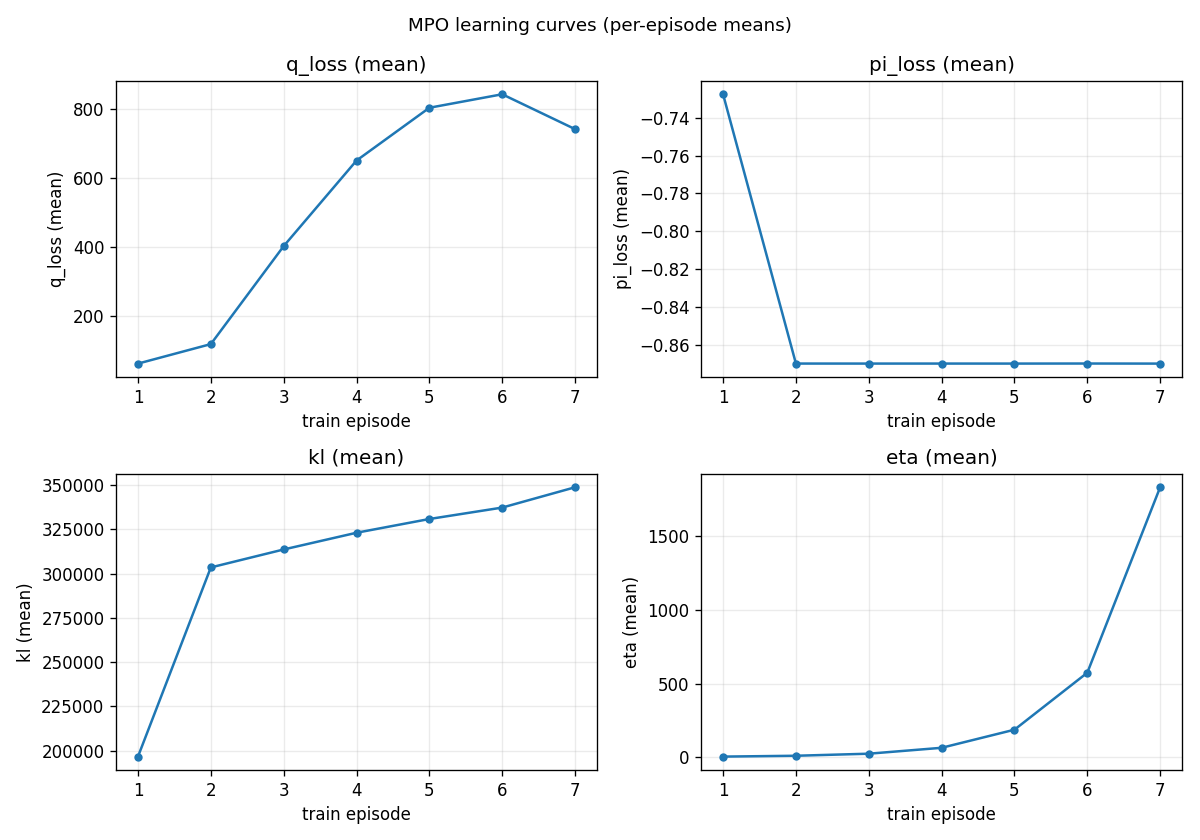
\includegraphics[width=\linewidth]{figures/fig_learning_curve_exp1.png}
    \caption{Exp~1 (not learning)}
  \end{subfigure}\hfill
  \begin{subfigure}[t]{0.48\linewidth}
    \centering
    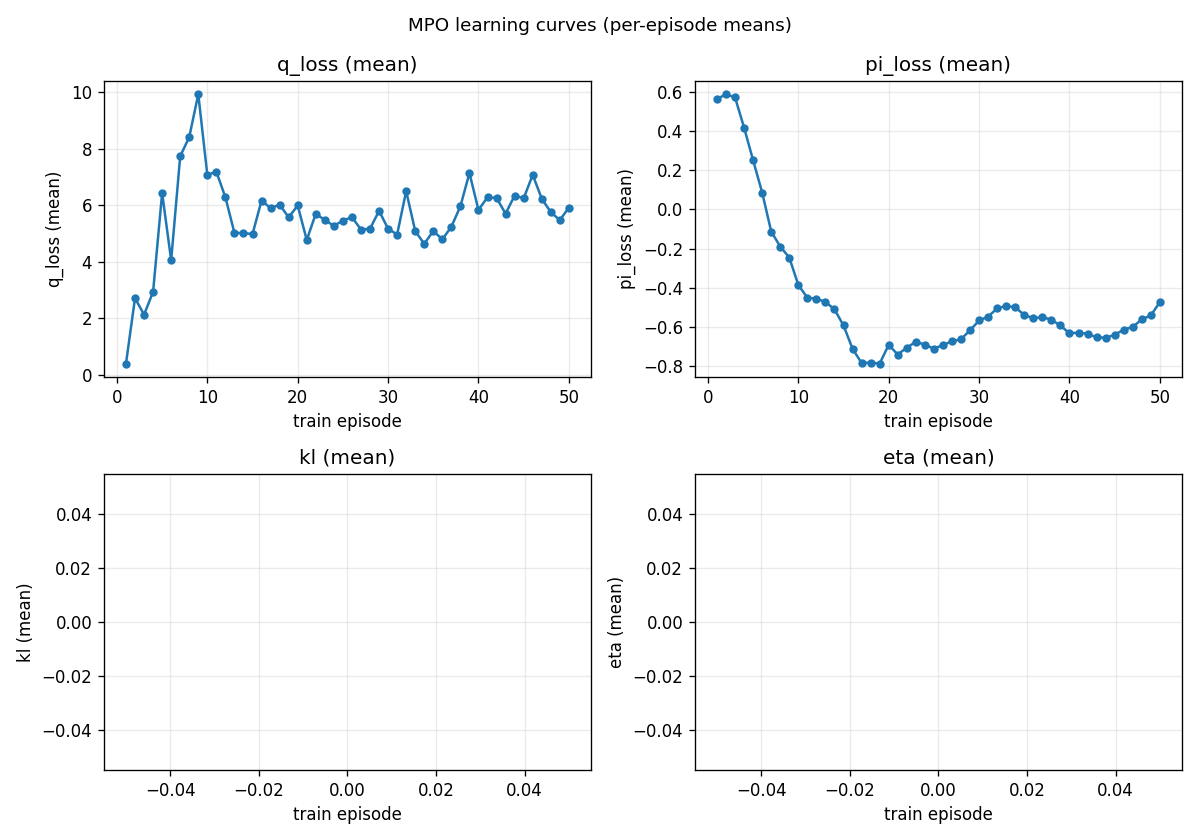
\includegraphics[width=\linewidth]{figures/fig_learning_curve_exp9.png}
    \caption{Exp~9 (learning)}
  \end{subfigure}
  \caption{Learning behaviour contrast: flat/collapsed training under Exp~1 shutter-threshold MPO versus rising returns under Exp~9 SAC shutter-split (best supported SAC configuration).}
  \label{fig:learning-vs-not}
\end{figure}

\begin{figure}[htbp]
  \centering
  \begin{subfigure}[t]{0.48\linewidth}
    \centering
    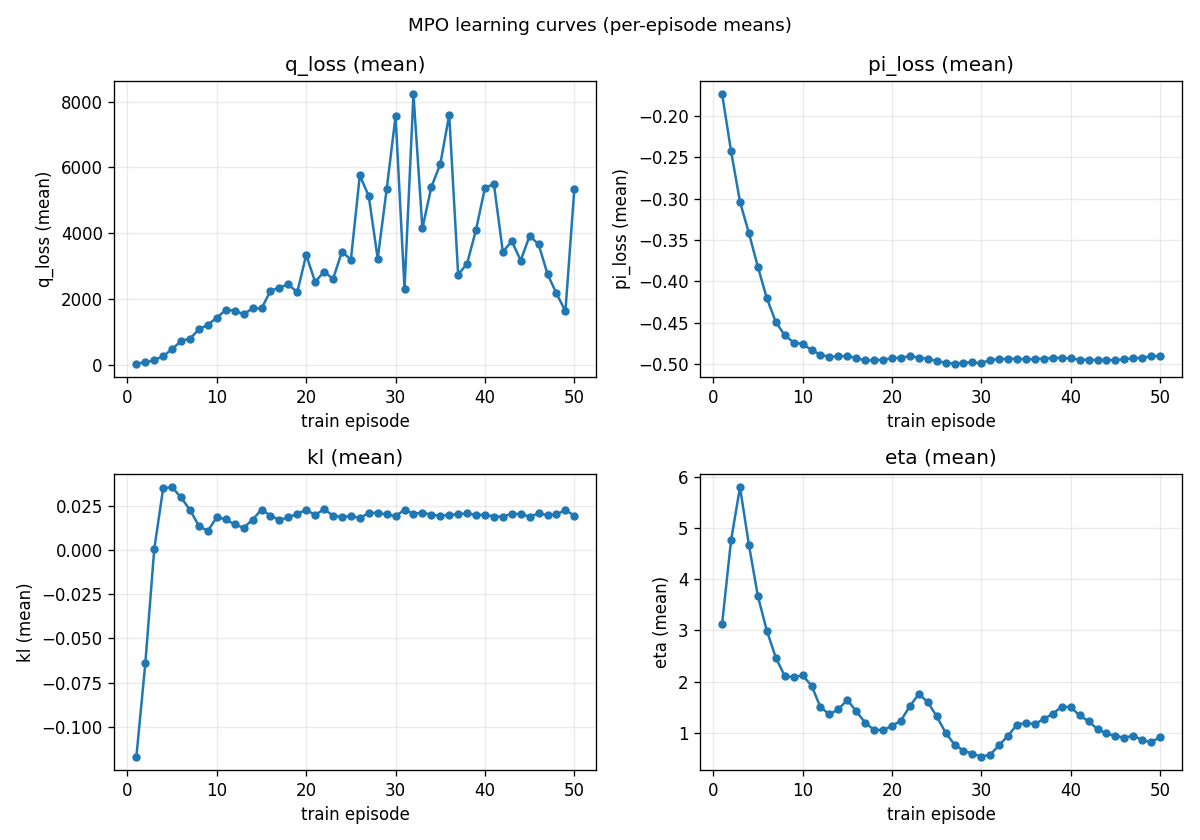
\includegraphics[width=\linewidth]{figures/fig_learning_curve_exp10.png}
    \caption{Exp~10 (not learning)}
  \end{subfigure}\hfill
  \begin{subfigure}[t]{0.48\linewidth}
    \centering
    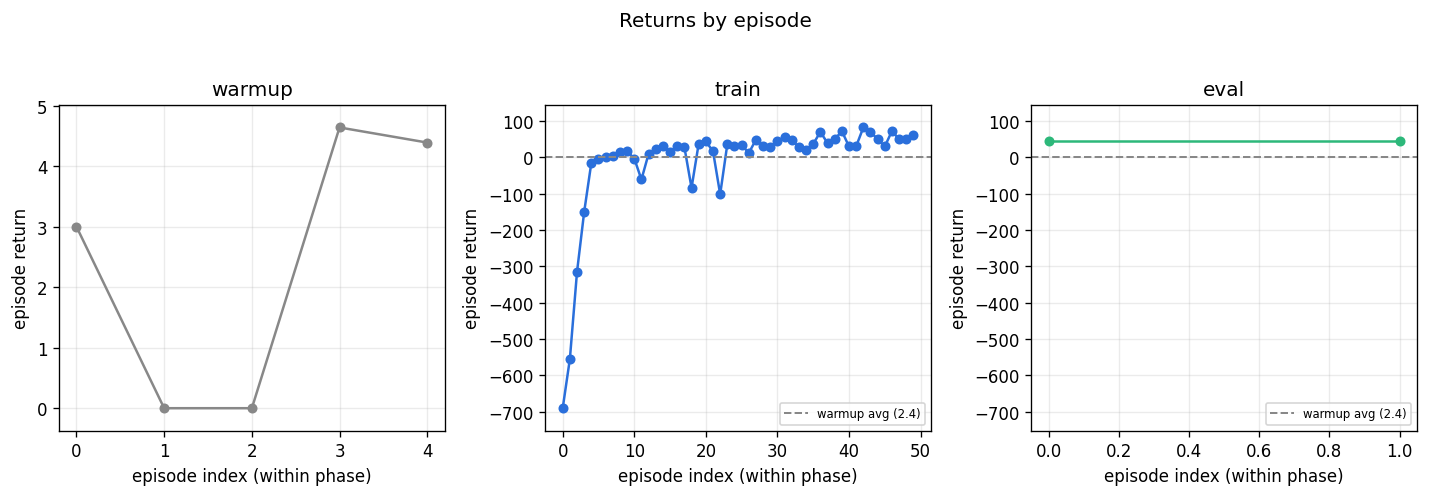
\includegraphics[width=\linewidth]{figures/fig_learning_curve_exp11.png}
    \caption{Exp~11 (learning)}
  \end{subfigure}
  \caption{MPO branch after the Exp~8 dual fix: Exp~10 safe-mode penalty collapses eval return, while Exp~11 vector-mode MPO shows sustained learning.}
  \label{fig:learning-mpo-contrast}
\end{figure}

\subsection{Shutter spam and budget efficiency}
\label{sec:results-shutter}

Shutter command count per episode tracks whether a policy has learned selective scheduling rather than firing continuously.
A well-trained policy would issue at most ten commands per episode (one per target within budget), timed to clear-sky windows.
The deterministic baseline issues exactly ten commands but ignores cloud content, so an estimated 30--40\% of its captures are wasted on cloud-blocked or empty targets.

Table~\ref{tab:shutter-progression} tracks the spam reduction path.

\begin{table}[htbp]
  \centering
  \caption{Shutter spam reduction across the SAC vector experiment chain.
    All figures are training means unless noted.}
  \label{tab:shutter-progression}
  \begin{tabular}{lrrl}
    \toprule
    Experiment & Cmds/ep (train) & Meaningful frac (train) & Notes \\
    \midrule
    Overnight H1a (pre-Exp~1) & 968 & 0 & MPO, threshold 0.5 \\
    Exp~1 mpo\_t05/t09         & 516 & 0 & Threshold ineffective \\
    Exp~4 Ref1 (SAC vector)    & 7071 & 0.015 & Budget ignorance \\
    Exp~7 (budget penalty)     & 478  & 0.220 & $-93\%$ cmds vs Ref1 \\
    Exp~9 (waste off)          & --- & 0.286 / 0.667 (eval) & Best scheduling \\
    Exp~11 (MPO vector)        & 8--10 & --- & Budget-aware MPO \\
    Baseline anchor (reference)  & 10  & $\sim$0.60--0.70 & Deterministic, cloud-blind \\
    \bottomrule
  \end{tabular}
\end{table}

The budget-exhausted penalty (Exp~7) was the single most impactful reward change in the series:
a 93\% reduction in shutter commands with a simultaneous increase in eval return.
Removing the waste penalty (Exp~9) added a further behavioural improvement on top of that configuration.
Together, these results show that reward structure, not algorithm choice alone, determines whether selective shuttering emerges.

\begin{figure}[htbp]
  \centering
  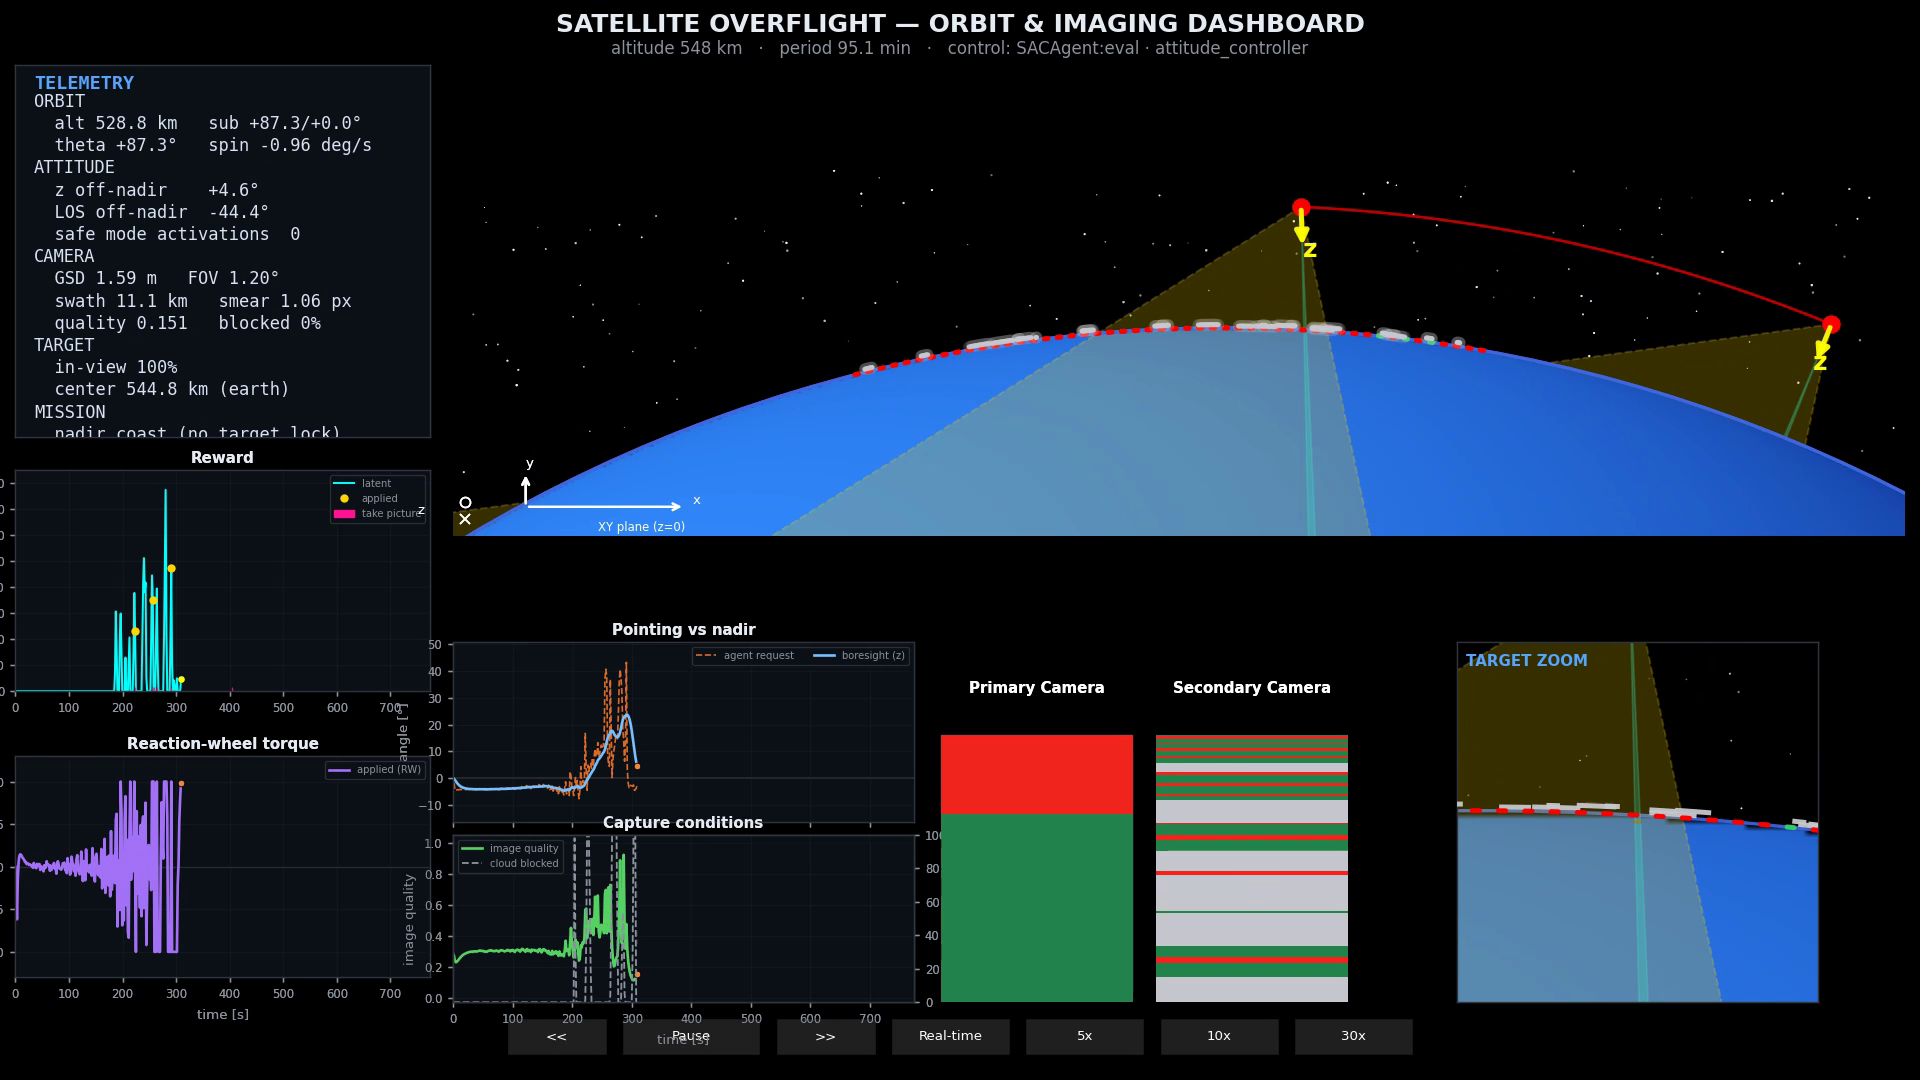
\includegraphics[width=0.88\linewidth]{figures/fig_selective_shutter.png}
  \caption{Eval episode from Exp~9 (SAC shutter-split): representative dashboard frame during selective capture behaviour on the fixed evaluation seed.}
  \label{fig:selective-shutter}
\end{figure}

\subsection{Safe-mode and safety overhead}
\label{sec:results-safemode}

In torque mode (Exps~1--5, 8) the safety controller activates 5--6 times per episode,
locking out the agent for 60\,s per event (Section~\ref{sec:safety}).
Each lockout consumes $\approx$40 controller steps with no capture opportunity.
With 516 steps per episode and 5 lockouts, approximately 40\% of the episode is unavailable to the agent.

Vector mode (Exps~4 Ref1, 7, 9, 11, 12) eliminates safe-mode lockouts in the experiment runs:
the hold-last semantics prevent the pointing reference from exceeding $\theta_\text{hard}$,
so the safety controller is never triggered.

This structural difference explains much of the torque-versus-vector gap.
The safe-mode penalty (Exp~10) attempted to replicate this improvement via reward shaping
but produced the worst result in the series ($-510.4$), confirming that action-space redesign (vector mode) is preferable to reward penalties for aligning safety and learning.

\subsection{Algorithm comparison: SAC vs.\ MPO}
\label{sec:results-algo}

At matched protocol (sparse, vector, 50 episodes, seed~7), the best SAC configuration (Exp~9, $+106.4$) exceeds the best MPO configuration (Exp~11, $+45.5$) on eval return by 60.9 points.
The gap is partially explained by reward configuration: Exp~9 uses the waste-off, budget-on reward while Exp~11 uses the budget-on, waste-on default.
An MPO run with the Exp~9 reward settings was not completed within the project timeline.

Both best configurations exceed the baseline anchor on this seed ($-38.6$).
That is encouraging for the design search but not sufficient evidence of robust mission-level superiority: evaluation uses only two episodes at a fixed seed, and several intermediate configurations never learned at all.
The more durable finding is behavioural.
Both algorithms can learn selective shuttering once reward and action-space choices are correct.
That is a stronger claim than reliable baseline outperformance under all training conditions.


\section{Discussion}
\label{sec:discussion}

\subsection{What the experiment sequence taught}
\label{sec:discussion-arc}

The motivating idea, use onboard vision to shutter only on clear targets, is simple to state but hard to train.
The fourteen experiments were not a single attempt to beat the baseline; they were a structured search for reward and action-space configurations that make learning possible.
Three lessons emerged.
Per-experiment returns and shutter counts are reported in Sections~\ref{sec:experiments} and~\ref{sec:results}; this subsection interprets why the levers mattered.

\paragraph{1.\ Reward structure before algorithm.}
Neither threshold tuning, encoder architecture, algorithm choice, nor network width was sufficient on its own.
Learning emerged only after the reward told the agent what mattered at the action clock: sparse capture credit, a budget-exhausted penalty that stops shutter spam, and removal of a redundant within-budget waste term.
Reward engineering was the dominant design lever; swapping algorithms without that structure did not unlock selective shuttering.

\paragraph{2.\ Action-space design before reward fine-tuning.}
Delegating rate control to the onboard pointing controller (vector mode) is structurally important relative to raw torque commands.
Vector mode removes safe-mode lockouts in the experiment runs (Section~\ref{sec:results-safemode}), resolving a credit-assignment problem that no reward penalty could fix cleanly.
This is a design result: the agent should command a pointing offset, not raw wheel torque, for cloud-aware scheduling in this environment (Section~\ref{sec:discussion-architecture}).

\paragraph{3.\ Algorithm stability as a prerequisite.}
An unconstrained MPO trust-region update blocked the MPO branch until the dual-variable bug was corrected.
After that fix, vector-mode MPO learned without a further reward redesign.
Implementation correctness can masquerade as algorithm failure; that check comes before comparing reward or action-space variants.

\subsection{Answer to the research question}
\label{sec:discussion-answer}

Cloud-aware autonomous scheduling is not trivial to train in this simulation.
A minimal viable training stack requires at least:
\begin{itemize}
  \item a sparse capture-credit reward with a budget-exhausted shutter penalty;
  \item vector pointing mode (nadir-relative offset) rather than direct torque commands;
  \item a correctly implemented MPO trust-region update, or SAC as the more forgiving default;
  \item baseline-policy warmup to seed the replay buffer with rare positive-credit transitions.
\end{itemize}
With that stack, both SAC and MPO learn selective shuttering absent in the deterministic baseline.
Several configurations that looked reasonable (threshold tuning, network width, safe-mode penalties, torque effort in vector mode) failed to produce learning or made it worse.
Eval return on seed~7 exceeded the matched average baseline return for the best SAC and MPO configurations, but the evaluation protocol is too narrow to claim robust mission superiority; the durable output of the semester is the mapped design space and the list of rejected shortcuts.

\subsection{Control hierarchy and action interface}
\label{sec:discussion-architecture}

Development did not begin with the interface the experiments ultimately recommend.

\paragraph{From torque to safety arbitration.}
The first experimental interface exposed raw reaction-wheel torque to the learning agent.
Unconstrained policies could command aggressive slews; in simulation this produced sustained rotation that would be unacceptable on flight hardware.
Review with system engineers motivated treating attitude safety as non-negotiable: every agent command, whether torque or pointing request, passes through a safety controller that can taper, reject, or replace commands with a safe-mode recovery sequence (Section~\ref{sec:safety}).
That stack is shared by the deterministic baseline and all learned policies.

\paragraph{Action modes tested.}
Three action interfaces were explored:
\begin{itemize}
  \item \textbf{Torque mode:} the policy commands wheel torque directly (Exps~1--5, 8, 10).
  \item \textbf{Vector mode:} the policy commands a nadir-relative pointing offset; the OBC converts it to PD torque (Exps~4, 7, 9, 11--13).
  \item \textbf{Target selection:} a higher-level discrete choice of which target to engage (Exp~14).
    Started as a hypothesised next simplification after torque and vector; the run did not complete, so whether this interface is easier to train remains open.
\end{itemize}

\paragraph{Segregation of control layers.}
The experiment arc supports separating what the agent should learn from what the OBC should execute.
Learning precise torque profiles or continuous pointing offsets is not the primary scheduling problem in this environment: the agent must decide \emph{when} to expose the shutter given cloud feedback, while rate control and maneuver execution belong downstream.
Vector mode reflects that split and improved learning in practice (Exps~4, 11).
A torque-trained agent might in principle discover rich low-level strategies, for example multiple captures within one forward-motion-compensation maneuver.
It is a further \emph{hypothesis}, not a result of this report, that raising the action interface to explicit target selection (plus shutter timing) would simplify credit assignment further; Exp~14 was begun on that conviction but time ran out before it could be validated, and implementation or gradient issues in that branch have not been ruled out.
Energy-optimal wheel commands remain a distinct optimisation problem; they should be trained or tuned in a separate low-level loop rather than entangled with cloud-aware target scheduling.

\paragraph{Intended end state (working hypothesis).}
A plausible long-term stack is three levels: mission intent from the ground or onboard planner, a vision-driven scheduling policy (target and shutter decisions), and OBC execution with PD pointing and hard safety limits.
Vector mode is the highest-level interface validated here; target selection is the candidate next step named above.
This semester maps the scheduling layer under vector actions in a simplified 2D simulator; the lowest layer is modelled but not co-trained for efficiency.

\subsection{Rejected paths}
\label{sec:discussion-rejected}

Table~\ref{tab:rejected} summarises design choices that were tested and ruled out.

\begin{table}[htbp]
  \centering
  \caption{Rejected experimental directions with rationale.}
  \label{tab:rejected}
  \begin{tabular}{p{0.22\linewidth}p{0.34\linewidth}p{0.36\linewidth}}
    \toprule
    Experiment & Design choice tested & Why rejected \\
    \midrule
    --- & MPC pointing controller & Superseded by onboard PD pointing; lower scope and comparable results \\
    --- & Latent-only dense reward & Dense reward tested at $10\times$ applied scale; did not unblock MPO \\
    Exp~1 & Shutter threshold 0.5 $\to$ 0.9 & Policy saturates shutter output regardless of threshold \\
    --- & 15\,s capture credit window & Latent bursts visible; applied capture remains zero \\
    Exp~5 & MPO network width ablation & Identical collapse at all widths; capacity not the bottleneck \\
    Exp~9 & Within-budget waste penalty (on) & Redundant with apply-credit sparsity; penalising same failure mode twice \\
    Exp~10 & Safe-mode penalty & Correlation with aggressive pointing suppresses useful captures \\
    Exp~12 & Torque effort in vector mode & Pointing-controller torque $\neq$ policy action; conflicting gradient \\
    \bottomrule
  \end{tabular}
\end{table}

\subsection{Limitations}
\label{sec:limitations}

\paragraph{Two-dimensional simulation.}
The entire dynamics model, camera model, and reward signal operate in a single orbit plane.
Real three-axis attitude control involves cross-coupling between roll, pitch, and yaw;
disturbance torques from solar pressure, magnetic field, and gravity gradient; and
three-dimensional off-nadir imaging geometry.
The 2D model provides a tractable learning environment but the policies are not directly
transferable to hardware.

\paragraph{Single-pass, single-orbit mission.}
Each episode models one overflight of a fixed 50-target corridor.
Revisit scheduling, downlink windows, and multi-orbit memory are not represented.
The learned policy has no access to observations from prior passes.

\paragraph{Simulation-only evaluation.}
No hardware-in-the-loop or software-in-the-loop tests were conducted.
The camera model is a geometric ray tracer with an analytic smear formula; radiometric calibration,
MTF, and sensor noise are absent.
Generalisation from this environment to a real EO instrument is an open question.

\paragraph{Fixed-seed evaluation.}
All primary eval returns are computed on two episodes at seed~7.
The train-to-eval gap visible in several experiments (e.g.\ Exp~9 train $+169.9$ vs eval $+106.4$)
may partially reflect evaluation seed dependence.
A robust evaluation across $\ge$10 seeds is recommended before citing the best numbers as
reliable performance estimates.

\paragraph{Budget and episode length.}
The 10-capture budget over 516 steps is an engineered constraint that simplifies mission planning
but may not represent realistic EO tasking where capture rate, data volume, and ground station contact
are coupled objectives.

\subsection{Deferred extensions}
\label{sec:discussion-deferred}

The following directions are documented as promising but were not completed within the project:

\begin{itemize}
  \item \textbf{Modular encoder rerun (deferred Exp~6).}
    Once learning is established, the vector-compressor encoder variant from Exp~2 should be retested.
    The high-dimensional observation with structured bearing and mask fields is
    a candidate for entity-based architectures \citep{gorishniy2022revisiting}.

  \item \textbf{MPO with Exp~9 reward config.}
    Exp~11 reached $+45.5$ without the waste-penalty-off configuration used in Exp~9.
    A direct MPO run at Exp~9 reward settings would quantify the algorithm gap more cleanly.

  \item \textbf{Target-selection interface (Exp~14 rerun).}
    Hypothesis: discrete target choice plus shutter timing delegates pointing entirely to the OBC and may simplify learning relative to vector mode.
    Exp~14 began testing this idea but crashed before a conclusive result; a rerun must also rule out implementation or gradient bugs in that branch, not only extend training time.

  \item \textbf{Three-axis attitude extension.}
    Moving from 2D to 3D dynamics is the prerequisite for any hardware-facing transfer.
    The simulation architecture supports this extension via replacement of the single-axis
    RW model with a 3-wheel assembly and attitude quaternion propagation.

  \item \textbf{Real imagery and radiometric reward.}
    Replacing the geometric smear quality metric with a model-based image quality score
    derived from sensor noise and scene contrast would couple the reward more directly
    to downstream science value.
\end{itemize}


\section{Conclusion}
\label{sec:conclusion}

We set out to answer a question that looks simple from the outside:
if cloud-aware autonomous scheduling is obviously better than a fixed capture plan, what reward shaping and action-space design are needed to train such a policy in simulation?
The semester work shows that the answer is not trivial.

A reproducible simulation and training platform was built to investigate that question systematically.
Fourteen experiments varied reward structure, action representation, and learning algorithm under matched baseline conditions.
Three design levers dominated the outcome: reward information at the action clock, delegating rate control to a pointing controller rather than raw torque commands, and correct implementation of the MPO trust-region update.
Once those were in place, both SAC and MPO developed selective shuttering behaviour absent in the deterministic baseline.
Reliable quantitative outperformance of that baseline on mission return was not established within the semester scope; the main contribution is a mapped design space and an experimental protocol for continuing the search.

\textbf{Outlook.}
Near-term work: extend evaluation beyond aggregate return, tighten the protocol for longer training runs, and migrate control authority toward mission-level intent while keeping a single canonical episode artifact for train, eval, and render.
Logical extensions beyond this semester include three-dimensional attitude and orbit propagation, richer terrain and real imagery ingestion, and multi-orbit scheduling.


\appendix
\section{Supplementary material}
\label{sec:appendix}

\subsection{Repository}
The full source code, experiment scripts, and run artifacts are available at:
\begin{center}
  \url{https://github.com/cgriede/autonomous-satellite-control-eth-sem-proj}
\end{center}

\subsection{Source index}
Table~\ref{tab:source-index} lists the high-level entry points for the components described in this report.
All paths are relative to the repository root.

\begin{table}[htbp]
  \centering
  \renewcommand{\arraystretch}{1.3}
  \caption{High-level source index.}
  \label{tab:source-index}
  \small
  \begin{tabular}{@{}>{\raggedright\arraybackslash}p{0.32\linewidth}>{\raggedright\arraybackslash}p{0.62\linewidth}@{}}
    \toprule
    Component & Entry point \\
    \midrule
    Earth \& geodetic constants & \path|backend/environment_definition/constants/EARTH.py| \\
    Mission profile (altitude, targets) & \path|backend/environment_definition/constants/MISSION.py| \\
    Satellite inertia \& camera optics & \path|backend/environment_definition/constants/SATELLITE.py| \\
    Attitude safety thresholds & \path|backend/environment_definition/constants/ATTITUDE_SAFETY.py| \\
    Simulation timing & \path|backend/environment_definition/constants/SIMULATION.py| \\
    Reward weights & \path|backend/environment_definition/constants/AUTONOMOUS_CONTROL_REWARD.py| \\
    Canonical simulation entry point & \path|backend/simulation/run_simulation.py| \\
    Camera image quality model & \path|backend/simulation/image_quality.py| \\
    Attitude safety controller & \path|backend/simulation/attitude_controller.py| \\
    Deterministic baseline policy & \path|backend/s01_utils/baseline_overflight.py| \\
    RL agent (MPO / SAC) & \path|backend/autonomous_control/controller_agent.py| \\
    Training workflow & \path|backend/autonomous_control/training_workflow.py| \\
    Experiment scripts & \path|backend/scripts/experiments/| \\
    Per-run return KPIs (warmup/train/eval) & \path|backend/autonomous_control/runs/<run-id>/summary_metrics.json| \\
    \bottomrule
  \end{tabular}
\end{table}

\subsection{Live parameter record}
Hyperparameters and constants are maintained in:
\begin{itemize}
  \item \path|docs/presentation/environment-hyperparameters.md|
  \item \path|docs/presentation/machine-learning.md|
  \item \path|docs/presentation/technical-constants.md|
  \item \path|docs/presentation/physical-reference.md|
\end{itemize}

\subsection{Artifact paths}
\begin{itemize}
  \item Training outputs: \path|backend/autonomous_control/runs/<run-id>/|
  \item Experiment results: \path|backend/scripts/experiments/<slug>/results/|
\end{itemize}


\bibliography{references}

\end{document}
